% Options for packages loaded elsewhere
\PassOptionsToPackage{unicode}{hyperref}
\PassOptionsToPackage{hyphens}{url}
%
\documentclass[
]{article}
\usepackage{lmodern}
\usepackage{amssymb,amsmath}
\usepackage{ifxetex,ifluatex}
\ifnum 0\ifxetex 1\fi\ifluatex 1\fi=0 % if pdftex
  \usepackage[T1]{fontenc}
  \usepackage[utf8]{inputenc}
  \usepackage{textcomp} % provide euro and other symbols
\else % if luatex or xetex
  \usepackage{unicode-math}
  \defaultfontfeatures{Scale=MatchLowercase}
  \defaultfontfeatures[\rmfamily]{Ligatures=TeX,Scale=1}
\fi
% Use upquote if available, for straight quotes in verbatim environments
\IfFileExists{upquote.sty}{\usepackage{upquote}}{}
\IfFileExists{microtype.sty}{% use microtype if available
  \usepackage[]{microtype}
  \UseMicrotypeSet[protrusion]{basicmath} % disable protrusion for tt fonts
}{}
\makeatletter
\@ifundefined{KOMAClassName}{% if non-KOMA class
  \IfFileExists{parskip.sty}{%
    \usepackage{parskip}
  }{% else
    \setlength{\parindent}{0pt}
    \setlength{\parskip}{6pt plus 2pt minus 1pt}}
}{% if KOMA class
  \KOMAoptions{parskip=half}}
\makeatother
\usepackage{xcolor}
\IfFileExists{xurl.sty}{\usepackage{xurl}}{} % add URL line breaks if available
\IfFileExists{bookmark.sty}{\usepackage{bookmark}}{\usepackage{hyperref}}
\hypersetup{
  pdftitle={HW1},
  pdfauthor={Zachary Palmore},
  hidelinks,
  pdfcreator={LaTeX via pandoc}}
\urlstyle{same} % disable monospaced font for URLs
\usepackage[margin=1in]{geometry}
\usepackage{color}
\usepackage{fancyvrb}
\newcommand{\VerbBar}{|}
\newcommand{\VERB}{\Verb[commandchars=\\\{\}]}
\DefineVerbatimEnvironment{Highlighting}{Verbatim}{commandchars=\\\{\}}
% Add ',fontsize=\small' for more characters per line
\usepackage{framed}
\definecolor{shadecolor}{RGB}{248,248,248}
\newenvironment{Shaded}{\begin{snugshade}}{\end{snugshade}}
\newcommand{\AlertTok}[1]{\textcolor[rgb]{0.94,0.16,0.16}{#1}}
\newcommand{\AnnotationTok}[1]{\textcolor[rgb]{0.56,0.35,0.01}{\textbf{\textit{#1}}}}
\newcommand{\AttributeTok}[1]{\textcolor[rgb]{0.77,0.63,0.00}{#1}}
\newcommand{\BaseNTok}[1]{\textcolor[rgb]{0.00,0.00,0.81}{#1}}
\newcommand{\BuiltInTok}[1]{#1}
\newcommand{\CharTok}[1]{\textcolor[rgb]{0.31,0.60,0.02}{#1}}
\newcommand{\CommentTok}[1]{\textcolor[rgb]{0.56,0.35,0.01}{\textit{#1}}}
\newcommand{\CommentVarTok}[1]{\textcolor[rgb]{0.56,0.35,0.01}{\textbf{\textit{#1}}}}
\newcommand{\ConstantTok}[1]{\textcolor[rgb]{0.00,0.00,0.00}{#1}}
\newcommand{\ControlFlowTok}[1]{\textcolor[rgb]{0.13,0.29,0.53}{\textbf{#1}}}
\newcommand{\DataTypeTok}[1]{\textcolor[rgb]{0.13,0.29,0.53}{#1}}
\newcommand{\DecValTok}[1]{\textcolor[rgb]{0.00,0.00,0.81}{#1}}
\newcommand{\DocumentationTok}[1]{\textcolor[rgb]{0.56,0.35,0.01}{\textbf{\textit{#1}}}}
\newcommand{\ErrorTok}[1]{\textcolor[rgb]{0.64,0.00,0.00}{\textbf{#1}}}
\newcommand{\ExtensionTok}[1]{#1}
\newcommand{\FloatTok}[1]{\textcolor[rgb]{0.00,0.00,0.81}{#1}}
\newcommand{\FunctionTok}[1]{\textcolor[rgb]{0.00,0.00,0.00}{#1}}
\newcommand{\ImportTok}[1]{#1}
\newcommand{\InformationTok}[1]{\textcolor[rgb]{0.56,0.35,0.01}{\textbf{\textit{#1}}}}
\newcommand{\KeywordTok}[1]{\textcolor[rgb]{0.13,0.29,0.53}{\textbf{#1}}}
\newcommand{\NormalTok}[1]{#1}
\newcommand{\OperatorTok}[1]{\textcolor[rgb]{0.81,0.36,0.00}{\textbf{#1}}}
\newcommand{\OtherTok}[1]{\textcolor[rgb]{0.56,0.35,0.01}{#1}}
\newcommand{\PreprocessorTok}[1]{\textcolor[rgb]{0.56,0.35,0.01}{\textit{#1}}}
\newcommand{\RegionMarkerTok}[1]{#1}
\newcommand{\SpecialCharTok}[1]{\textcolor[rgb]{0.00,0.00,0.00}{#1}}
\newcommand{\SpecialStringTok}[1]{\textcolor[rgb]{0.31,0.60,0.02}{#1}}
\newcommand{\StringTok}[1]{\textcolor[rgb]{0.31,0.60,0.02}{#1}}
\newcommand{\VariableTok}[1]{\textcolor[rgb]{0.00,0.00,0.00}{#1}}
\newcommand{\VerbatimStringTok}[1]{\textcolor[rgb]{0.31,0.60,0.02}{#1}}
\newcommand{\WarningTok}[1]{\textcolor[rgb]{0.56,0.35,0.01}{\textbf{\textit{#1}}}}
\usepackage{graphicx}
\makeatletter
\def\maxwidth{\ifdim\Gin@nat@width>\linewidth\linewidth\else\Gin@nat@width\fi}
\def\maxheight{\ifdim\Gin@nat@height>\textheight\textheight\else\Gin@nat@height\fi}
\makeatother
% Scale images if necessary, so that they will not overflow the page
% margins by default, and it is still possible to overwrite the defaults
% using explicit options in \includegraphics[width, height, ...]{}
\setkeys{Gin}{width=\maxwidth,height=\maxheight,keepaspectratio}
% Set default figure placement to htbp
\makeatletter
\def\fps@figure{htbp}
\makeatother
\setlength{\emergencystretch}{3em} % prevent overfull lines
\providecommand{\tightlist}{%
  \setlength{\itemsep}{0pt}\setlength{\parskip}{0pt}}
\setcounter{secnumdepth}{-\maxdimen} % remove section numbering
\newcommand{\bcenter}{\begin{center}}
\newcommand{\ecenter}{\end{center}}
\usepackage{booktabs}
\usepackage{longtable}
\usepackage{array}
\usepackage{multirow}
\usepackage{wrapfig}
\usepackage{float}
\usepackage{colortbl}
\usepackage{pdflscape}
\usepackage{tabu}
\usepackage{threeparttable}
\usepackage{threeparttablex}
\usepackage[normalem]{ulem}
\usepackage{makecell}
\usepackage{xcolor}
\ifluatex
  \usepackage{selnolig}  % disable illegal ligatures
\fi

\title{HW1}
\usepackage{etoolbox}
\makeatletter
\providecommand{\subtitle}[1]{% add subtitle to \maketitle
  \apptocmd{\@title}{\par {\large #1 \par}}{}{}
}
\makeatother
\subtitle{Business Analytics and Data Mining}
\author{Zachary Palmore}
\date{2/15/2021}

\begin{document}
\maketitle

\begin{center}

\hypertarget{assignment-1}{%
\section{Assignment 1}\label{assignment-1}}

\end{center}

\hypertarget{purpose}{%
\subsection{Purpose}\label{purpose}}

Our purpose is to design a linear regression model that makes the best
prediction about how many games a baseball team can win in a season. The
best way to do that today is with the training data set provided. In
this analysis we are going to explore performance statistics from an MLB
team, evaluate their performance, and make predictions about their
winnings.

\hypertarget{data-exploration}{%
\subsection{Data Exploration}\label{data-exploration}}

\hypertarget{background}{%
\subsubsection{Background}\label{background}}

\begin{Shaded}
\begin{Highlighting}[]
\CommentTok{\# Packages }
\FunctionTok{library}\NormalTok{(tidyverse)}
\FunctionTok{library}\NormalTok{(ggpubr)}
\FunctionTok{library}\NormalTok{(kableExtra)}
\FunctionTok{library}\NormalTok{(reshape2)}
\FunctionTok{library}\NormalTok{(corrplot)}
\FunctionTok{library}\NormalTok{(ggstatsplot)}
\FunctionTok{library}\NormalTok{(MASS)}
\FunctionTok{library}\NormalTok{(bestNormalize)}
\FunctionTok{library}\NormalTok{(Metrics)}
\FunctionTok{library}\NormalTok{(VGAM)}
\FunctionTok{theme\_set}\NormalTok{(}\FunctionTok{theme\_minimal}\NormalTok{())}
\end{Highlighting}
\end{Shaded}

\begin{Shaded}
\begin{Highlighting}[]
\CommentTok{\# Our training data}
\NormalTok{tdata }\OtherTok{\textless{}{-}} \FunctionTok{read.csv}\NormalTok{(}
\StringTok{"https://raw.githubusercontent.com/palmorezm/data621/main/moneyball{-}training{-}data.csv}
\StringTok{?token=AQYT6MZMRA4GRVITJM7BRUDAGVK7G"}\NormalTok{)}
\CommentTok{\# Basic statistics from the set }
\NormalTok{total.obs }\OtherTok{\textless{}{-}} \FunctionTok{count}\NormalTok{(tdata)}
\NormalTok{avg.wins }\OtherTok{\textless{}{-}} \FunctionTok{mean}\NormalTok{(tdata}\SpecialCharTok{$}\NormalTok{TARGET\_WINS) }
\NormalTok{max.wins }\OtherTok{\textless{}{-}} \FunctionTok{max}\NormalTok{(tdata}\SpecialCharTok{$}\NormalTok{TARGET\_WINS)}
\NormalTok{sd.wins }\OtherTok{\textless{}{-}} \FunctionTok{sd}\NormalTok{(tdata}\SpecialCharTok{$}\NormalTok{TARGET\_WINS)}
\NormalTok{colnames }\OtherTok{\textless{}{-}} \FunctionTok{colnames}\NormalTok{(tdata)}
\NormalTok{missing.values }\OtherTok{\textless{}{-}}\NormalTok{ (}\FunctionTok{sum}\NormalTok{(}\FunctionTok{is.na}\NormalTok{(tdata)))}
\end{Highlighting}
\end{Shaded}

In this data set, there are 2276 observations of a major league baseball
team from 1871 to 2006. These statistics have been adjusted to match the
typical performance of a 162-game season and no team has won every game
in a season. A sample of the data is provided for reference.

\begin{Shaded}
\begin{Highlighting}[]
\CommentTok{\# create samples of table data}
\NormalTok{tdata.tbl}\FloatTok{.1} \OtherTok{\textless{}{-}}\NormalTok{ tdata[}\DecValTok{1}\SpecialCharTok{:}\DecValTok{5}\NormalTok{,}\FunctionTok{c}\NormalTok{(}\DecValTok{1}\SpecialCharTok{:}\DecValTok{4}\NormalTok{, }\DecValTok{17}\NormalTok{)]}
\NormalTok{tdata.tbl}\FloatTok{.2} \OtherTok{\textless{}{-}}\NormalTok{ tdata[}\DecValTok{1}\SpecialCharTok{:}\DecValTok{5}\NormalTok{,}\DecValTok{5}\SpecialCharTok{:}\DecValTok{8}\NormalTok{]}
\NormalTok{tdata.tbl}\FloatTok{.3} \OtherTok{\textless{}{-}}\NormalTok{ tdata[}\DecValTok{1}\SpecialCharTok{:}\DecValTok{5}\NormalTok{,}\DecValTok{9}\SpecialCharTok{:}\DecValTok{12}\NormalTok{]}
\NormalTok{tdata.tbl}\FloatTok{.4} \OtherTok{\textless{}{-}}\NormalTok{ tdata[}\DecValTok{1}\SpecialCharTok{:}\DecValTok{5}\NormalTok{,}\DecValTok{13}\SpecialCharTok{:}\DecValTok{16}\NormalTok{]}
\CommentTok{\# display samples of table data}
\NormalTok{ttbl}\FloatTok{.1} \OtherTok{\textless{}{-}} \FunctionTok{kbl}\NormalTok{(tdata.tbl}\FloatTok{.1}\NormalTok{, }\AttributeTok{booktabs =}\NormalTok{ T, }\AttributeTok{caption =} \StringTok{"Training Data Fields 1 {-} 4 and 17"}\NormalTok{) }\SpecialCharTok{\%\textgreater{}\%}
  \FunctionTok{kable\_styling}\NormalTok{(}\AttributeTok{latex\_options =} \FunctionTok{c}\NormalTok{(}\StringTok{"striped"}\NormalTok{, }\StringTok{"hold\_position"}\NormalTok{),}
  \AttributeTok{full\_width =}\NormalTok{ F) }
\NormalTok{ttbl}\FloatTok{.2} \OtherTok{\textless{}{-}} \FunctionTok{kbl}\NormalTok{(tdata.tbl}\FloatTok{.2}\NormalTok{, }\AttributeTok{booktabs =}\NormalTok{ T, }\AttributeTok{caption =} \StringTok{"Training Data Fields 5 {-} 8"}\NormalTok{) }\SpecialCharTok{\%\textgreater{}\%}
  \FunctionTok{kable\_styling}\NormalTok{(}\AttributeTok{latex\_options =} \FunctionTok{c}\NormalTok{(}\StringTok{"striped"}\NormalTok{, }\StringTok{"hold\_position"}\NormalTok{),}
  \AttributeTok{full\_width =}\NormalTok{ F) }
\NormalTok{ttbl}\FloatTok{.3} \OtherTok{\textless{}{-}} \FunctionTok{kbl}\NormalTok{(tdata.tbl}\FloatTok{.3}\NormalTok{, }\AttributeTok{booktabs =}\NormalTok{ T, }\AttributeTok{caption =} \StringTok{"Training Data Fields 9 {-} 12"}\NormalTok{) }\SpecialCharTok{\%\textgreater{}\%}
  \FunctionTok{kable\_styling}\NormalTok{(}\AttributeTok{latex\_options =} \FunctionTok{c}\NormalTok{(}\StringTok{"striped"}\NormalTok{, }\StringTok{"hold\_position"}\NormalTok{),}
  \AttributeTok{full\_width =}\NormalTok{ F) }
\NormalTok{ttbl}\FloatTok{.4} \OtherTok{\textless{}{-}} \FunctionTok{kbl}\NormalTok{(tdata.tbl}\FloatTok{.4}\NormalTok{, }\AttributeTok{booktabs =}\NormalTok{ T, }\AttributeTok{caption =} \StringTok{"Training Data Fields 13 {-} 16"}\NormalTok{) }\SpecialCharTok{\%\textgreater{}\%}
  \FunctionTok{kable\_styling}\NormalTok{(}\AttributeTok{latex\_options =} \FunctionTok{c}\NormalTok{(}\StringTok{"striped"}\NormalTok{, }\StringTok{"hold\_position"}\NormalTok{),}
  \AttributeTok{full\_width =}\NormalTok{ F) }
\end{Highlighting}
\end{Shaded}

\begin{Shaded}
\begin{Highlighting}[]
\NormalTok{ttbl}\FloatTok{.1} 
\end{Highlighting}
\end{Shaded}

\begin{table}[!h]

\caption{\label{tab:unnamed-chunk-3}Training Data Fields 1 - 4 and 17}
\centering
\begin{tabular}[t]{rrrrr}
\toprule
INDEX & TARGET\_WINS & TEAM\_BATTING\_H & TEAM\_BATTING\_2B & TEAM\_FIELDING\_DP\\
\midrule
\cellcolor{gray!6}{1} & \cellcolor{gray!6}{39} & \cellcolor{gray!6}{1445} & \cellcolor{gray!6}{194} & \cellcolor{gray!6}{NA}\\
2 & 70 & 1339 & 219 & 155\\
\cellcolor{gray!6}{3} & \cellcolor{gray!6}{86} & \cellcolor{gray!6}{1377} & \cellcolor{gray!6}{232} & \cellcolor{gray!6}{153}\\
4 & 70 & 1387 & 209 & 156\\
\cellcolor{gray!6}{5} & \cellcolor{gray!6}{82} & \cellcolor{gray!6}{1297} & \cellcolor{gray!6}{186} & \cellcolor{gray!6}{168}\\
\bottomrule
\end{tabular}
\end{table}

\begin{Shaded}
\begin{Highlighting}[]
\NormalTok{ttbl}\FloatTok{.2} 
\end{Highlighting}
\end{Shaded}

\begin{table}[!h]

\caption{\label{tab:unnamed-chunk-3}Training Data Fields 5 - 8}
\centering
\begin{tabular}[t]{rrrr}
\toprule
TEAM\_BATTING\_3B & TEAM\_BATTING\_HR & TEAM\_BATTING\_BB & TEAM\_BATTING\_SO\\
\midrule
\cellcolor{gray!6}{39} & \cellcolor{gray!6}{13} & \cellcolor{gray!6}{143} & \cellcolor{gray!6}{842}\\
22 & 190 & 685 & 1075\\
\cellcolor{gray!6}{35} & \cellcolor{gray!6}{137} & \cellcolor{gray!6}{602} & \cellcolor{gray!6}{917}\\
38 & 96 & 451 & 922\\
\cellcolor{gray!6}{27} & \cellcolor{gray!6}{102} & \cellcolor{gray!6}{472} & \cellcolor{gray!6}{920}\\
\bottomrule
\end{tabular}
\end{table}

\begin{Shaded}
\begin{Highlighting}[]
\NormalTok{ttbl}\FloatTok{.3}
\end{Highlighting}
\end{Shaded}

\begin{table}[!h]

\caption{\label{tab:unnamed-chunk-3}Training Data Fields 9 - 12}
\centering
\begin{tabular}[t]{rrrr}
\toprule
TEAM\_BASERUN\_SB & TEAM\_BASERUN\_CS & TEAM\_BATTING\_HBP & TEAM\_PITCHING\_H\\
\midrule
\cellcolor{gray!6}{NA} & \cellcolor{gray!6}{NA} & \cellcolor{gray!6}{NA} & \cellcolor{gray!6}{9364}\\
37 & 28 & NA & 1347\\
\cellcolor{gray!6}{46} & \cellcolor{gray!6}{27} & \cellcolor{gray!6}{NA} & \cellcolor{gray!6}{1377}\\
43 & 30 & NA & 1396\\
\cellcolor{gray!6}{49} & \cellcolor{gray!6}{39} & \cellcolor{gray!6}{NA} & \cellcolor{gray!6}{1297}\\
\bottomrule
\end{tabular}
\end{table}

\begin{Shaded}
\begin{Highlighting}[]
\NormalTok{ttbl}\FloatTok{.4}
\end{Highlighting}
\end{Shaded}

\begin{table}[!h]

\caption{\label{tab:unnamed-chunk-3}Training Data Fields 13 - 16}
\centering
\begin{tabular}[t]{rrrr}
\toprule
TEAM\_PITCHING\_HR & TEAM\_PITCHING\_BB & TEAM\_PITCHING\_SO & TEAM\_FIELDING\_E\\
\midrule
\cellcolor{gray!6}{84} & \cellcolor{gray!6}{927} & \cellcolor{gray!6}{5456} & \cellcolor{gray!6}{1011}\\
191 & 689 & 1082 & 193\\
\cellcolor{gray!6}{137} & \cellcolor{gray!6}{602} & \cellcolor{gray!6}{917} & \cellcolor{gray!6}{175}\\
97 & 454 & 928 & 164\\
\cellcolor{gray!6}{102} & \cellcolor{gray!6}{472} & \cellcolor{gray!6}{920} & \cellcolor{gray!6}{138}\\
\bottomrule
\end{tabular}
\end{table}

There are 17 variables and of course, our target variable is called
TARGET\_WINS representing the number of wins for this team. We check for
outliers and overall patterns in the distributions of each variable. We
exclude the index value since it is not a performance statistic, only a
placeholder. This will tell us how to proceed in cleaning the data and
give us a sense of how normal these data are. At this time, we do not
need any labels as we are only looking at overall patterns.

\begin{Shaded}
\begin{Highlighting}[]
\CommentTok{\# Function to calculate and set pointrange}
\NormalTok{xysdu }\OtherTok{\textless{}{-}} \ControlFlowTok{function}\NormalTok{(x) \{}
\NormalTok{   m }\OtherTok{\textless{}{-}} \FunctionTok{mean}\NormalTok{(x)}
\NormalTok{   ymin }\OtherTok{\textless{}{-}}\NormalTok{ m }\SpecialCharTok{{-}} \FunctionTok{sd}\NormalTok{(x)}
\NormalTok{   ymax }\OtherTok{\textless{}{-}}\NormalTok{ m }\SpecialCharTok{+} \FunctionTok{sd}\NormalTok{(x)}
   \FunctionTok{return}\NormalTok{(}\FunctionTok{c}\NormalTok{(}\AttributeTok{y =}\NormalTok{ m, }\AttributeTok{ymin =}\NormalTok{ ymin, }\AttributeTok{ymax =}\NormalTok{ ymax))}
\NormalTok{\}}

\CommentTok{\# Organize data in buckets of similar distribution and scale}
\NormalTok{df }\OtherTok{\textless{}{-}}\NormalTok{ tdata }\SpecialCharTok{\%\textgreater{}\%}
       \FunctionTok{melt}\NormalTok{() }\SpecialCharTok{\%\textgreater{}\%} 
       \FunctionTok{filter}\NormalTok{(variable }\SpecialCharTok{!=} \FunctionTok{c}\NormalTok{(}\StringTok{"INDEX"}\NormalTok{))}
\NormalTok{df1 }\OtherTok{\textless{}{-}}\NormalTok{ tdata }\SpecialCharTok{\%\textgreater{}\%}
       \FunctionTok{melt}\NormalTok{() }\SpecialCharTok{\%\textgreater{}\%} 
       \FunctionTok{filter}\NormalTok{(variable }\SpecialCharTok{==} \FunctionTok{c}\NormalTok{(}\StringTok{"TARGET\_WINS"}\NormalTok{, }
                       \StringTok{"TEAM\_BATTING\_H"}\NormalTok{, }
                       \StringTok{"TEAM\_BATTING\_2B"}\NormalTok{,}
                       \StringTok{"TEAM\_BATTING\_3B"}\NormalTok{))}
\NormalTok{df2 }\OtherTok{\textless{}{-}}\NormalTok{ tdata }\SpecialCharTok{\%\textgreater{}\%}
       \FunctionTok{melt}\NormalTok{() }\SpecialCharTok{\%\textgreater{}\%} 
       \FunctionTok{filter}\NormalTok{(variable }\SpecialCharTok{==} \FunctionTok{c}\NormalTok{(}\StringTok{"TEAM\_BATTING\_HR"}\NormalTok{, }
                       \StringTok{"TEAM\_BATTING\_BB"}\NormalTok{,}
                       \StringTok{"TEAM\_FIELDING\_E"}\NormalTok{,}
                       \StringTok{"TEAM\_FIELDING\_DP"}\NormalTok{))}
\NormalTok{df3 }\OtherTok{\textless{}{-}}\NormalTok{ tdata }\SpecialCharTok{\%\textgreater{}\%}
       \FunctionTok{melt}\NormalTok{() }\SpecialCharTok{\%\textgreater{}\%} 
       \FunctionTok{filter}\NormalTok{(variable }\SpecialCharTok{==} \FunctionTok{c}\NormalTok{(}\StringTok{"TEAM\_BASERUN\_CS"}\NormalTok{, }
                       \StringTok{"TEAM\_BATTING\_HBP"}\NormalTok{, }
                       \StringTok{"TEAM\_BASERUN\_SB"}\NormalTok{,}
                       \StringTok{"TEAM\_PITCHING\_HR"}\NormalTok{))}
\NormalTok{df4 }\OtherTok{\textless{}{-}}\NormalTok{ tdata }\SpecialCharTok{\%\textgreater{}\%}
  \FunctionTok{melt}\NormalTok{() }\SpecialCharTok{\%\textgreater{}\%} 
  \FunctionTok{filter}\NormalTok{(variable }\SpecialCharTok{==} \FunctionTok{c}\NormalTok{(}\StringTok{"TEAM\_PITCHING\_BB"}\NormalTok{, }
                       \StringTok{"TEAM\_PITCHING\_SO"}\NormalTok{, }
                       \StringTok{"TEAM\_BATTING\_SO"}\NormalTok{,}
                       \StringTok{"TEAM\_PITCHING\_H"}\NormalTok{))}

\CommentTok{\# Violin plots}
\NormalTok{vplt.df1 }\OtherTok{\textless{}{-}} \FunctionTok{ggplot}\NormalTok{(df1, }\FunctionTok{aes}\NormalTok{(variable, value)) }\SpecialCharTok{+} 
  \FunctionTok{geom\_violin}\NormalTok{(}\AttributeTok{trim =} \ConstantTok{FALSE}\NormalTok{, }\AttributeTok{scale=}\StringTok{"area"}\NormalTok{, }
              \FunctionTok{aes}\NormalTok{(}\AttributeTok{color=}\NormalTok{variable, }\AttributeTok{fill=}\NormalTok{variable, }\AttributeTok{alpha=}\FloatTok{0.15}\NormalTok{, )) }\SpecialCharTok{+} \FunctionTok{coord\_flip}\NormalTok{() }\SpecialCharTok{+} 
  \FunctionTok{geom\_boxplot}\NormalTok{(}\AttributeTok{width=}\NormalTok{.}\DecValTok{05}\NormalTok{, }\AttributeTok{shape=}\DecValTok{1}\NormalTok{, }\AttributeTok{alpha=}\FloatTok{0.20}\NormalTok{, }\AttributeTok{color=}\StringTok{"black"}\NormalTok{, }\AttributeTok{size=}\NormalTok{.}\DecValTok{5}\NormalTok{) }\SpecialCharTok{+} 
  \FunctionTok{theme}\NormalTok{(}\AttributeTok{legend.position =} \StringTok{"None"}\NormalTok{, }
        \AttributeTok{axis.title.x =} \FunctionTok{element\_blank}\NormalTok{(), }
        \AttributeTok{axis.title.y =} \FunctionTok{element\_blank}\NormalTok{(), }\AttributeTok{axis.text.y =} \FunctionTok{element\_blank}\NormalTok{())}

\NormalTok{vplt.df2 }\OtherTok{\textless{}{-}} \FunctionTok{ggplot}\NormalTok{(df2, }\FunctionTok{aes}\NormalTok{(variable, value)) }\SpecialCharTok{+} 
  \FunctionTok{geom\_violin}\NormalTok{(}\AttributeTok{trim =} \ConstantTok{FALSE}\NormalTok{, }\AttributeTok{scale=}\StringTok{"area"}\NormalTok{, }
              \FunctionTok{aes}\NormalTok{(}\AttributeTok{color=}\NormalTok{variable, }\AttributeTok{fill=}\NormalTok{variable, }\AttributeTok{alpha=}\FloatTok{0.15}\NormalTok{, )) }\SpecialCharTok{+} \FunctionTok{coord\_flip}\NormalTok{() }\SpecialCharTok{+} 
  \FunctionTok{geom\_boxplot}\NormalTok{(}\AttributeTok{width=}\NormalTok{.}\DecValTok{05}\NormalTok{, }\AttributeTok{shape=}\DecValTok{1}\NormalTok{, }\AttributeTok{alpha=}\FloatTok{0.20}\NormalTok{, }\AttributeTok{color=}\StringTok{"black"}\NormalTok{, }\AttributeTok{size=}\NormalTok{.}\DecValTok{5}\NormalTok{) }\SpecialCharTok{+} 
  \FunctionTok{theme}\NormalTok{(}\AttributeTok{legend.position =} \StringTok{"None"}\NormalTok{, }
        \AttributeTok{axis.title.x =} \FunctionTok{element\_blank}\NormalTok{(), }
        \AttributeTok{axis.title.y =} \FunctionTok{element\_blank}\NormalTok{(), }\AttributeTok{axis.text.y =} \FunctionTok{element\_blank}\NormalTok{())}

\NormalTok{vplt.df3 }\OtherTok{\textless{}{-}} \FunctionTok{ggplot}\NormalTok{(df3, }\FunctionTok{aes}\NormalTok{(variable, value)) }\SpecialCharTok{+} 
  \FunctionTok{geom\_violin}\NormalTok{(}\AttributeTok{trim =} \ConstantTok{FALSE}\NormalTok{, }\AttributeTok{scale=}\StringTok{"area"}\NormalTok{, }
              \FunctionTok{aes}\NormalTok{(}\AttributeTok{color=}\NormalTok{variable, }\AttributeTok{fill=}\NormalTok{variable, }\AttributeTok{alpha=}\FloatTok{0.15}\NormalTok{, )) }\SpecialCharTok{+} \FunctionTok{coord\_flip}\NormalTok{() }\SpecialCharTok{+} 
  \FunctionTok{geom\_boxplot}\NormalTok{(}\AttributeTok{width=}\NormalTok{.}\DecValTok{05}\NormalTok{, }\AttributeTok{shape=}\DecValTok{1}\NormalTok{, }\AttributeTok{alpha=}\FloatTok{0.20}\NormalTok{, }\AttributeTok{color=}\StringTok{"black"}\NormalTok{, }\AttributeTok{size=}\NormalTok{.}\DecValTok{5}\NormalTok{) }\SpecialCharTok{+} 
  \FunctionTok{theme}\NormalTok{(}\AttributeTok{legend.position =} \StringTok{"None"}\NormalTok{, }
        \AttributeTok{axis.title.x =} \FunctionTok{element\_blank}\NormalTok{(), }
        \AttributeTok{axis.title.y =} \FunctionTok{element\_blank}\NormalTok{(), }\AttributeTok{axis.text.y =} \FunctionTok{element\_blank}\NormalTok{())}

\NormalTok{vplt.df4 }\OtherTok{\textless{}{-}} \FunctionTok{ggplot}\NormalTok{(df4, }\FunctionTok{aes}\NormalTok{(variable, value)) }\SpecialCharTok{+} 
  \FunctionTok{geom\_violin}\NormalTok{(}\AttributeTok{trim =} \ConstantTok{FALSE}\NormalTok{, }\AttributeTok{scale=}\StringTok{"area"}\NormalTok{, }
              \FunctionTok{aes}\NormalTok{(}\AttributeTok{color=}\NormalTok{variable, }\AttributeTok{fill=}\NormalTok{variable, }\AttributeTok{alpha=}\FloatTok{0.15}\NormalTok{, )) }\SpecialCharTok{+} \FunctionTok{coord\_flip}\NormalTok{() }\SpecialCharTok{+} 
  \FunctionTok{geom\_boxplot}\NormalTok{(}\AttributeTok{width=}\NormalTok{.}\DecValTok{05}\NormalTok{, }\AttributeTok{shape=}\DecValTok{1}\NormalTok{, }\AttributeTok{alpha=}\FloatTok{0.20}\NormalTok{, }\AttributeTok{color=}\StringTok{"black"}\NormalTok{, }\AttributeTok{size=}\NormalTok{.}\DecValTok{5}\NormalTok{) }\SpecialCharTok{+} 
  \FunctionTok{theme}\NormalTok{(}\AttributeTok{legend.position =} \StringTok{"None"}\NormalTok{, }
        \AttributeTok{axis.title.x =} \FunctionTok{element\_blank}\NormalTok{(), }
        \AttributeTok{axis.title.y =} \FunctionTok{element\_blank}\NormalTok{(), }\AttributeTok{axis.text.y =} \FunctionTok{element\_blank}\NormalTok{())}


\CommentTok{\# Pointrange mean and median distribution}
\NormalTok{ptrangeplt.df1 }\OtherTok{\textless{}{-}} \FunctionTok{ggplot}\NormalTok{(df1, }\FunctionTok{aes}\NormalTok{(variable, value)) }\SpecialCharTok{+} \FunctionTok{coord\_flip}\NormalTok{() }\SpecialCharTok{+} 
  \FunctionTok{stat\_summary}\NormalTok{(}\AttributeTok{fun.data=}\NormalTok{xysdu, }\AttributeTok{geom =} \StringTok{"Pointrange"}\NormalTok{, }\AttributeTok{shape=}\DecValTok{16}\NormalTok{, }\AttributeTok{size=}\NormalTok{.}\DecValTok{5}\NormalTok{, }\AttributeTok{color=}\StringTok{"black"}\NormalTok{) }\SpecialCharTok{+}
  \FunctionTok{stat\_summary}\NormalTok{(}\AttributeTok{fun.y=}\NormalTok{median, }\AttributeTok{geom=}\StringTok{"point"}\NormalTok{, }\AttributeTok{shape=}\DecValTok{16}\NormalTok{, }\AttributeTok{size=}\DecValTok{2}\NormalTok{, }\AttributeTok{color=}\StringTok{"red"}\NormalTok{) }\SpecialCharTok{+} 
  \FunctionTok{theme}\NormalTok{(}\AttributeTok{legend.position =} \StringTok{"None"}\NormalTok{, }\AttributeTok{axis.title.x =} \FunctionTok{element\_blank}\NormalTok{(), }\AttributeTok{axis.title.y =} \FunctionTok{element\_blank}\NormalTok{())}

\NormalTok{ptrangeplt.df2 }\OtherTok{\textless{}{-}} \FunctionTok{ggplot}\NormalTok{(df2, }\FunctionTok{aes}\NormalTok{(variable, value)) }\SpecialCharTok{+} \FunctionTok{coord\_flip}\NormalTok{() }\SpecialCharTok{+} 
  \FunctionTok{stat\_summary}\NormalTok{(}\AttributeTok{fun.data=}\NormalTok{xysdu, }\AttributeTok{geom =} \StringTok{"Pointrange"}\NormalTok{, }\AttributeTok{shape=}\DecValTok{16}\NormalTok{, }\AttributeTok{size=}\NormalTok{.}\DecValTok{5}\NormalTok{, }\AttributeTok{color=}\StringTok{"black"}\NormalTok{) }\SpecialCharTok{+}
  \FunctionTok{stat\_summary}\NormalTok{(}\AttributeTok{fun.y=}\NormalTok{median, }\AttributeTok{geom=}\StringTok{"point"}\NormalTok{, }\AttributeTok{shape=}\DecValTok{16}\NormalTok{, }\AttributeTok{size=}\DecValTok{2}\NormalTok{, }\AttributeTok{color=}\StringTok{"red"}\NormalTok{) }\SpecialCharTok{+} 
  \FunctionTok{theme}\NormalTok{(}\AttributeTok{legend.position =} \StringTok{"None"}\NormalTok{, }\AttributeTok{axis.title.x =} \FunctionTok{element\_blank}\NormalTok{(), }\AttributeTok{axis.title.y =} \FunctionTok{element\_blank}\NormalTok{())}

\NormalTok{ptrangeplt.df3 }\OtherTok{\textless{}{-}} \FunctionTok{ggplot}\NormalTok{(df3, }\FunctionTok{aes}\NormalTok{(variable, value)) }\SpecialCharTok{+} \FunctionTok{coord\_flip}\NormalTok{() }\SpecialCharTok{+} 
  \FunctionTok{stat\_summary}\NormalTok{(}\AttributeTok{fun.data=}\NormalTok{xysdu, }\AttributeTok{geom =} \StringTok{"Pointrange"}\NormalTok{, }\AttributeTok{shape=}\DecValTok{16}\NormalTok{, }\AttributeTok{size=}\NormalTok{.}\DecValTok{5}\NormalTok{, }\AttributeTok{color=}\StringTok{"black"}\NormalTok{) }\SpecialCharTok{+}
  \FunctionTok{stat\_summary}\NormalTok{(}\AttributeTok{fun.y=}\NormalTok{median, }\AttributeTok{geom=}\StringTok{"point"}\NormalTok{, }\AttributeTok{shape=}\DecValTok{16}\NormalTok{, }\AttributeTok{size=}\DecValTok{2}\NormalTok{, }\AttributeTok{color=}\StringTok{"red"}\NormalTok{) }\SpecialCharTok{+} 
  \FunctionTok{theme}\NormalTok{(}\AttributeTok{legend.position =} \StringTok{"None"}\NormalTok{, }\AttributeTok{axis.title.x =} \FunctionTok{element\_blank}\NormalTok{(), }\AttributeTok{axis.title.y =} \FunctionTok{element\_blank}\NormalTok{())}

\NormalTok{ptrangeplt.df4 }\OtherTok{\textless{}{-}} \FunctionTok{ggplot}\NormalTok{(df4, }\FunctionTok{aes}\NormalTok{(variable, value)) }\SpecialCharTok{+} \FunctionTok{coord\_flip}\NormalTok{() }\SpecialCharTok{+} 
  \FunctionTok{stat\_summary}\NormalTok{(}\AttributeTok{fun.data=}\NormalTok{xysdu, }\AttributeTok{geom =} \StringTok{"Pointrange"}\NormalTok{, }\AttributeTok{shape=}\DecValTok{16}\NormalTok{, }\AttributeTok{size=}\NormalTok{.}\DecValTok{5}\NormalTok{, }\AttributeTok{color=}\StringTok{"black"}\NormalTok{) }\SpecialCharTok{+}
  \FunctionTok{stat\_summary}\NormalTok{(}\AttributeTok{fun.y=}\NormalTok{median, }\AttributeTok{geom=}\StringTok{"point"}\NormalTok{, }\AttributeTok{shape=}\DecValTok{16}\NormalTok{, }\AttributeTok{size=}\DecValTok{2}\NormalTok{, }\AttributeTok{color=}\StringTok{"red"}\NormalTok{) }\SpecialCharTok{+} 
  \FunctionTok{theme}\NormalTok{(}\AttributeTok{legend.position =} \StringTok{"None"}\NormalTok{, }
        \AttributeTok{axis.title.x =} \FunctionTok{element\_blank}\NormalTok{(), }\AttributeTok{axis.title.y =} \FunctionTok{element\_blank}\NormalTok{())}

\NormalTok{garnge.vplts.area }\OtherTok{\textless{}{-}} \FunctionTok{ggarrange}\NormalTok{(vplt.df1, vplt.df2, vplt.df3, vplt.df4)}
\NormalTok{garnge.ptrangeplts }\OtherTok{\textless{}{-}} \FunctionTok{ggarrange}\NormalTok{(ptrangeplt.df1, ptrangeplt.df2, ptrangeplt.df3, ptrangeplt.df4)}
\NormalTok{garnge.vplts.area }
\end{Highlighting}
\end{Shaded}

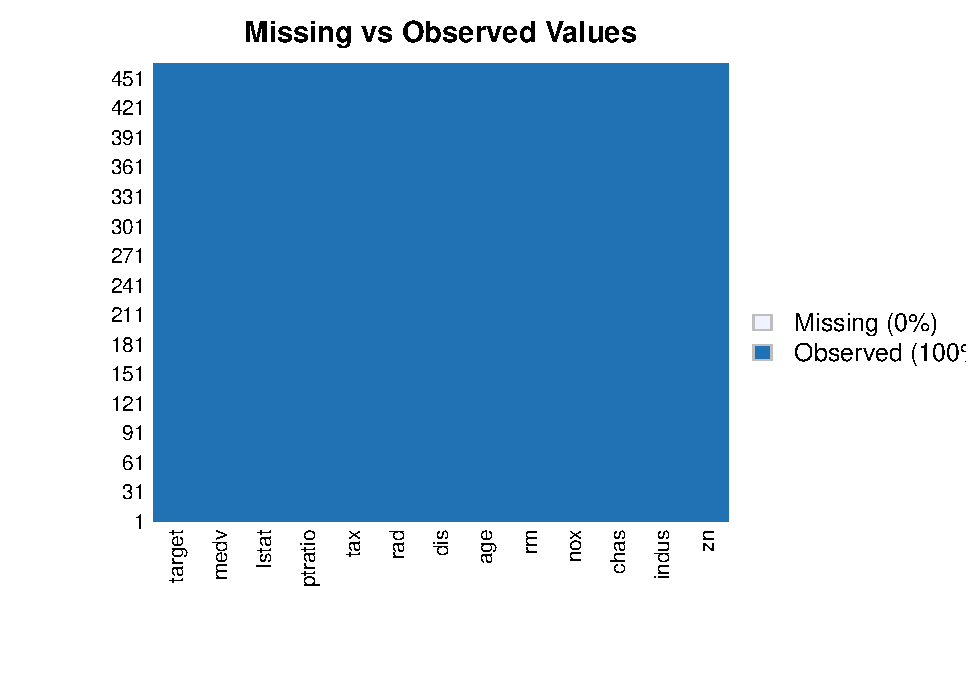
\includegraphics{HW1_files/figure-latex/unnamed-chunk-5-1.pdf}

This shows the distribution of each variable by kernel probability
density indicating where each variable is most likely to occur. There
are also black dots displayed within and along the colored probability
density lines to indicate outliers. From this we can gather that there
are many outliers and some are much larger and more frequent than
others. We can also see that there are a few potential predictors that
have little to no outliers and may be normal distributions. This is
great but to know if they can help the model, we check the magnitude of
outliers by exploiting the difference in robustness between median and
mean.

\begin{Shaded}
\begin{Highlighting}[]
\NormalTok{garnge.ptrangeplts }
\end{Highlighting}
\end{Shaded}

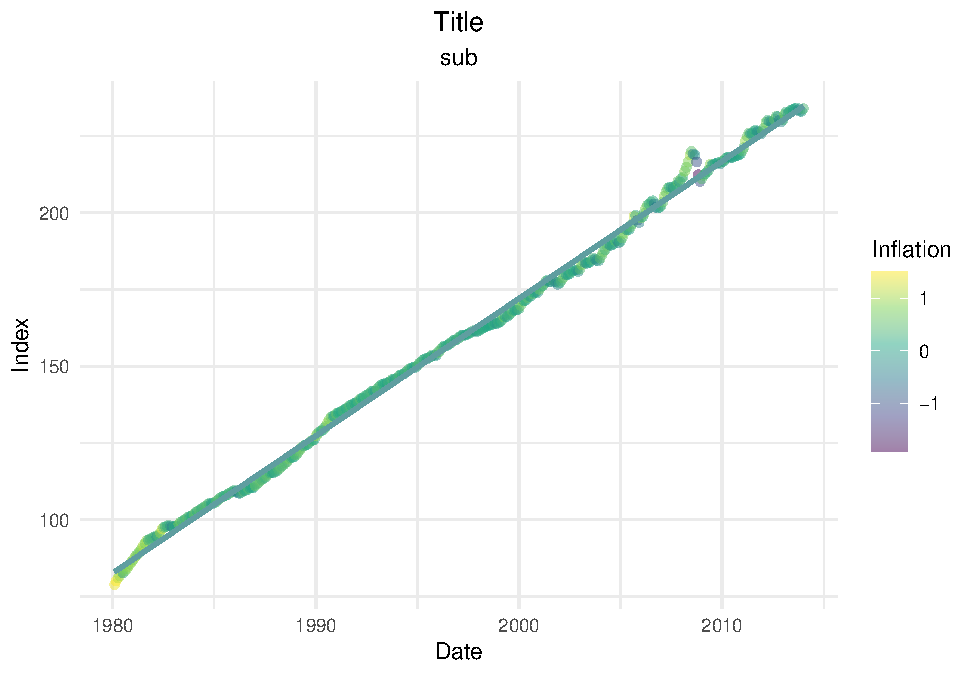
\includegraphics{HW1_files/figure-latex/unnamed-chunk-6-1.pdf}

When evaluating in this way, the variables' medians are plotted as red
dots on a black line that is the point range calculated from the
standard deviation of each distribution. In the center of that point
range is a black dot that represents the mean of each variable. The
farther away the red and black dots are from one another, the more
influence outliers have on the variable.

We can see from the chart that there are a lot of outliers and the scale
at which each occurs varies in magnitude from less than 1 to greater
than 50 points. These outliers must be dealt with prior to the analysis
if we are to use them to make predictions with. Otherwise, the models
will be skewed and the results will not be as accurate. For now, we
continue exploring the data.

\hypertarget{hypothesis}{%
\subsubsection{Hypothesis}\label{hypothesis}}

The average number of wins to a team is about 81 while the highest
number of wins recorded for a team at 146 in a season. Note that, these
calculations do not include any missing values nor outliers which should
make them reasonably representative of the real-world. Recall that our
main goal is to use this data to predict the number of wins for the
team.

Our expectation is that the number of wins will correlate best with
hits, home runs, fielding errors, and pitching strikeouts to produce a
linear model that is capable of predicting whether a team will win with
over 50\% accuracy. With that, we are making some assumptions about the
model, especially regarding TARGET\_WINS which records the number of
wins each season. These assumptions include normality in the
distribution, linearity, independence among events, and
homoscedasticity. With these assumptions satisfied, we can confirm that
it is reasonable to make predictions using the number of wins as our
target variable through proofs.

For purposes of this analysis, we accept the idea that each event must
be independent of one another since a statistic about one player does
not imply that we know any statistics about another player, nor the
entire team. Rather, we assume that a combination of performance
statistics about each player over time, can inform us about how well the
team will fare in future seasons. With that acceptance, we have our
first proof; independence among events.

The other conditional assumptions of linearity, normality, and
homoscedasticity can be proven using visualizations. Starting with
linearity, we intend to demonstrate that all of these variables are able
to be represented by a linear pattern. For this, an array of scatter
plots is shown with a linear trend overlaying the performance
statistics.

\begin{Shaded}
\begin{Highlighting}[]
\NormalTok{tdata[}\DecValTok{2}\SpecialCharTok{:}\DecValTok{17}\NormalTok{]  }\SpecialCharTok{\%\textgreater{}\%}
  \FunctionTok{gather}\NormalTok{(variable, value, }\SpecialCharTok{{-}}\NormalTok{TARGET\_WINS) }\SpecialCharTok{\%\textgreater{}\%} 
  \FunctionTok{ggplot}\NormalTok{(., }\FunctionTok{aes}\NormalTok{(value, TARGET\_WINS)) }\SpecialCharTok{+} 
  \FunctionTok{ggtitle}\NormalTok{(}\StringTok{"Linearity of Values"}\NormalTok{) }\SpecialCharTok{+} 
  \FunctionTok{geom\_point}\NormalTok{(}\AttributeTok{fill =} \StringTok{"white"}\NormalTok{,}
             \AttributeTok{size=}\DecValTok{1}\NormalTok{, }
             \AttributeTok{shape=}\DecValTok{1}\NormalTok{, }
             \AttributeTok{color=}\StringTok{"light blue"}\NormalTok{) }\SpecialCharTok{+} 
  \FunctionTok{geom\_smooth}\NormalTok{(}\AttributeTok{formula =}\NormalTok{ y}\SpecialCharTok{\textasciitilde{}}\NormalTok{x, }
              \AttributeTok{method =} \StringTok{"lm"}\NormalTok{, }
              \AttributeTok{size=}\NormalTok{.}\DecValTok{1}\NormalTok{,}
              \AttributeTok{se =} \ConstantTok{TRUE}\NormalTok{,}
              \AttributeTok{color =} \StringTok{"black"}\NormalTok{, }
              \AttributeTok{linetype =} \StringTok{"dotdash"}\NormalTok{, }
              \AttributeTok{alpha=}\FloatTok{0.25}\NormalTok{) }\SpecialCharTok{+} 
  \FunctionTok{facet\_wrap}\NormalTok{(}\SpecialCharTok{\textasciitilde{}}\NormalTok{variable, }
             \AttributeTok{scales =}\StringTok{"free"}\NormalTok{,}
             \AttributeTok{ncol =} \DecValTok{4}\NormalTok{) }\SpecialCharTok{+}
  \FunctionTok{theme}\NormalTok{(}\AttributeTok{axis.text.x =} \FunctionTok{element\_blank}\NormalTok{(), }\AttributeTok{axis.text.y =} \FunctionTok{element\_blank}\NormalTok{())}
\end{Highlighting}
\end{Shaded}

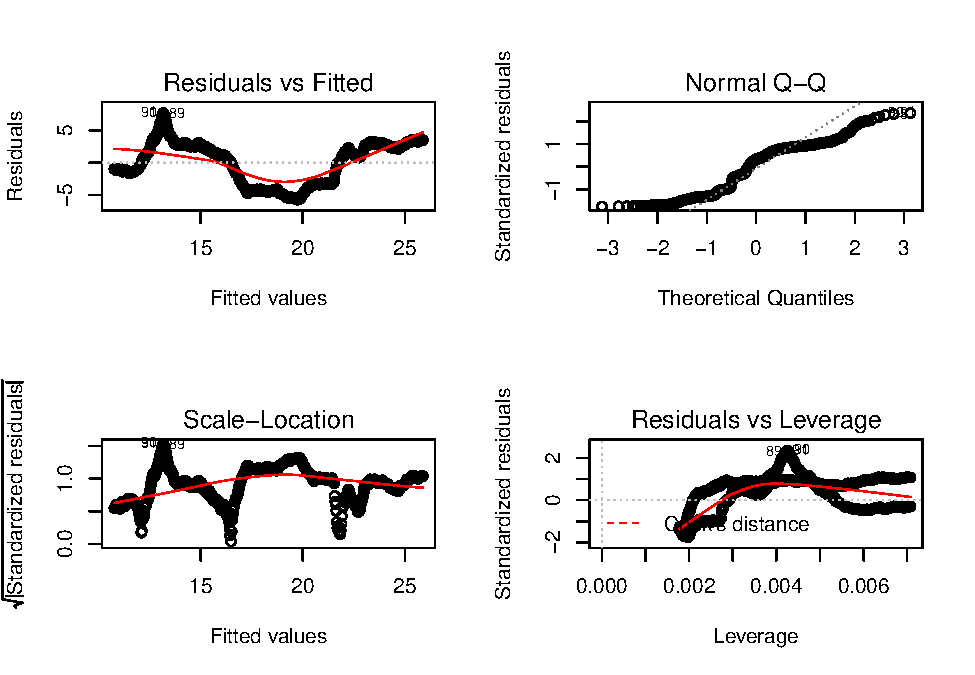
\includegraphics{HW1_files/figure-latex/unnamed-chunk-7-1.pdf}

While this includes the outliers mentioned previously, it is reasonable
to assume that almost all of these variables could be predicted using
linear trends. The only potential non-linear variables are
TEAM\_FIELDING\_E, TEAM\_PITCHING\_BB, TEAM\_PITCHING\_H, and
TEAM\_PITCHING\_SO. At first glance, these look like they might fit best
with another kind of model. But, with outliers removed and perhaps a
normalizing transformation we may alter the fit enough for their
prediction potential (and subsequent correlation with wins) to improve
model results.

Intentionally, we also do not know which correlations will be useful for
the model at this point. To decide on them now would not be helpful as
we are unsure of their efficacy in any linear model. Thus, we continue
validating these assumptions to build the models properly.

Normality is another assumption that we must ensure is present to make
accurate predictions with linear regression. It can be viewed and
confirmed in several ways but here we use a density plot to search for
smooth bell-curves and limited skewness.

\begin{Shaded}
\begin{Highlighting}[]
\NormalTok{tdata }\SpecialCharTok{\%\textgreater{}\%}
  \FunctionTok{gather}\NormalTok{(variable, value, TARGET\_WINS}\SpecialCharTok{:}\NormalTok{TEAM\_FIELDING\_DP) }\SpecialCharTok{\%\textgreater{}\%}
  \FunctionTok{ggplot}\NormalTok{(., }\FunctionTok{aes}\NormalTok{(value))  }\SpecialCharTok{+} 
  \FunctionTok{ggtitle}\NormalTok{(}\StringTok{"Distribution of Performance Variables"}\NormalTok{) }\SpecialCharTok{+} 
  \FunctionTok{geom\_density}\NormalTok{(}\AttributeTok{fill =} \StringTok{"white"}\NormalTok{, }\AttributeTok{color=}\StringTok{"lightblue"}\NormalTok{) }\SpecialCharTok{+} 
  \FunctionTok{labs}\NormalTok{(}\AttributeTok{x =} \FunctionTok{element\_blank}\NormalTok{(), }\AttributeTok{y =} \FunctionTok{element\_blank}\NormalTok{()) }\SpecialCharTok{+} 
  \FunctionTok{facet\_wrap}\NormalTok{(}\SpecialCharTok{\textasciitilde{}}\NormalTok{variable, }\AttributeTok{scales =}\StringTok{"free"}\NormalTok{, }\AttributeTok{ncol =} \DecValTok{4}\NormalTok{) }\SpecialCharTok{+}
  \FunctionTok{theme}\NormalTok{(}\AttributeTok{axis.text.x =} \FunctionTok{element\_blank}\NormalTok{(), }\AttributeTok{axis.text.y =} \FunctionTok{element\_blank}\NormalTok{())}
\end{Highlighting}
\end{Shaded}

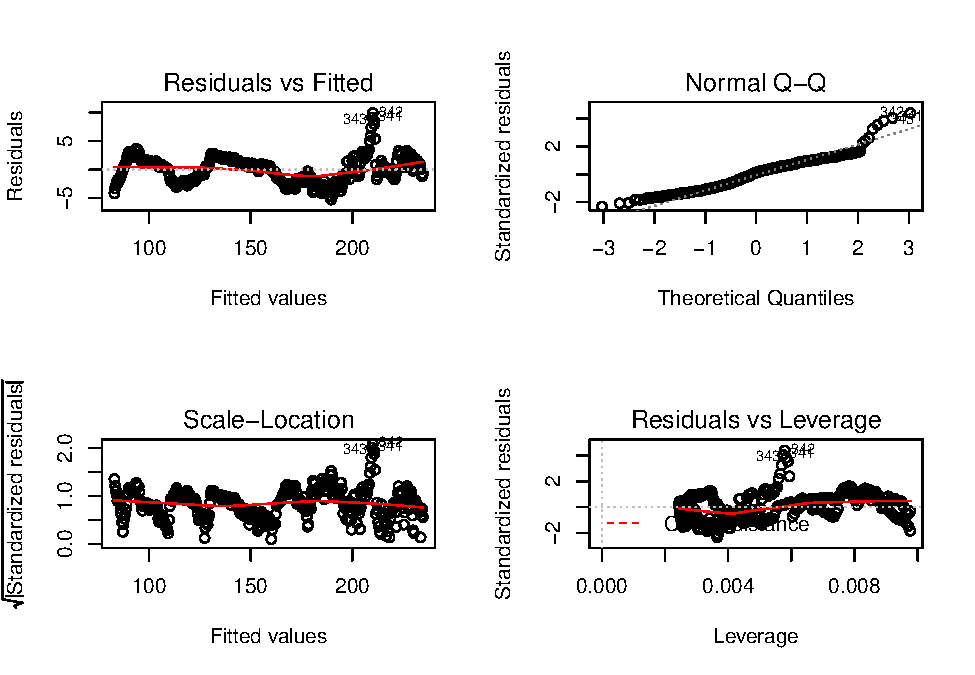
\includegraphics{HW1_files/figure-latex/unnamed-chunk-8-1.pdf}

Those same potential predictors that exhibited a nonlinear trend are
causing problems. As individual predictors of game wins they do not
appear normal. This could be caused entirely by outliers but we will
have to take a closer look at all the variables to identify the cause of
their variation. For this, we run a simple linear model that contains
all variables except the index to see how they interact together. In
doing so we also check for homoscedasticity, or consistency in variance
among the variables.

\begin{Shaded}
\begin{Highlighting}[]
\NormalTok{ks.test }\OtherTok{\textless{}{-}} \FunctionTok{lm}\NormalTok{(TARGET\_WINS }\SpecialCharTok{\textasciitilde{}}\NormalTok{. }\SpecialCharTok{{-}}\NormalTok{INDEX, tdata)}
\FunctionTok{summary}\NormalTok{(ks.test)}
\end{Highlighting}
\end{Shaded}

\begin{verbatim}
## 
## Call:
## lm(formula = TARGET_WINS ~ . - INDEX, data = tdata)
## 
## Residuals:
##      Min       1Q   Median       3Q      Max 
## -19.8708  -5.6564  -0.0599   5.2545  22.9274 
## 
## Coefficients:
##                  Estimate Std. Error t value Pr(>|t|)    
## (Intercept)      60.28826   19.67842   3.064  0.00253 ** 
## TEAM_BATTING_H    1.91348    2.76139   0.693  0.48927    
## TEAM_BATTING_2B   0.02639    0.03029   0.871  0.38484    
## TEAM_BATTING_3B  -0.10118    0.07751  -1.305  0.19348    
## TEAM_BATTING_HR  -4.84371   10.50851  -0.461  0.64542    
## TEAM_BATTING_BB  -4.45969    3.63624  -1.226  0.22167    
## TEAM_BATTING_SO   0.34196    2.59876   0.132  0.89546    
## TEAM_BASERUN_SB   0.03304    0.02867   1.152  0.25071    
## TEAM_BASERUN_CS  -0.01104    0.07143  -0.155  0.87730    
## TEAM_BATTING_HBP  0.08247    0.04960   1.663  0.09815 .  
## TEAM_PITCHING_H  -1.89096    2.76095  -0.685  0.49432    
## TEAM_PITCHING_HR  4.93043   10.50664   0.469  0.63946    
## TEAM_PITCHING_BB  4.51089    3.63372   1.241  0.21612    
## TEAM_PITCHING_SO -0.37364    2.59705  -0.144  0.88577    
## TEAM_FIELDING_E  -0.17204    0.04140  -4.155 5.08e-05 ***
## TEAM_FIELDING_DP -0.10819    0.03654  -2.961  0.00349 ** 
## ---
## Signif. codes:  0 '***' 0.001 '**' 0.01 '*' 0.05 '.' 0.1 ' ' 1
## 
## Residual standard error: 8.467 on 175 degrees of freedom
##   (2085 observations deleted due to missingness)
## Multiple R-squared:  0.5501, Adjusted R-squared:  0.5116 
## F-statistic: 14.27 on 15 and 175 DF,  p-value: < 2.2e-16
\end{verbatim}

\begin{Shaded}
\begin{Highlighting}[]
\FunctionTok{plot}\NormalTok{(ks.test)}
\end{Highlighting}
\end{Shaded}

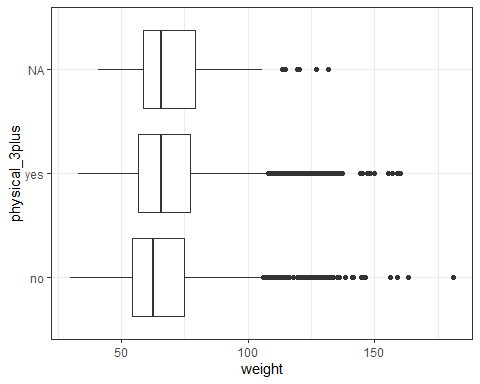
\includegraphics{HW1_files/figure-latex/unnamed-chunk-9-1.pdf}
\includegraphics{HW1_files/figure-latex/unnamed-chunk-9-2.pdf}
\includegraphics{HW1_files/figure-latex/unnamed-chunk-9-3.pdf}
\includegraphics{HW1_files/figure-latex/unnamed-chunk-9-4.pdf}

\begin{Shaded}
\begin{Highlighting}[]
\FunctionTok{hist}\NormalTok{(}\FunctionTok{resid}\NormalTok{(ks.test), }\AttributeTok{main=}\StringTok{"Distribution of Residuals"}\NormalTok{)}
\end{Highlighting}
\end{Shaded}

\includegraphics{HW1_files/figure-latex/unnamed-chunk-9-5.pdf}

Represented by the standardized residuals the homoscedasticity
assumption is confirmed. There is constant variance among the random
variables. However, normality seems to have slightly fixed itself when
considering all variables. As an added bonus to viewing this kind of
model, it reveals patterns of interaction with the variables and their
strengths. This model would be good enough to run on its own, but we
should continue to consider how it could be improved for data
preparation. We should fix missing variables, reduce high leverage
points, and make at least one transformation on those problem variables
even though our assumptions are closely met.

\hypertarget{predictor-correlations}{%
\subsubsection{Predictor Correlations}\label{predictor-correlations}}

To determine which variables could prove to be the best predictors of
game wins, it is important to consider the strength and direction of
correlation. For a quick look at how each variable compares with each
other, this correlation plot was built using only complete observations.

\begin{Shaded}
\begin{Highlighting}[]
\NormalTok{tdata[}\DecValTok{2}\SpecialCharTok{:}\DecValTok{17}\NormalTok{] }\SpecialCharTok{\%\textgreater{}\%}
  \FunctionTok{cor}\NormalTok{(., }\AttributeTok{use =} \StringTok{"complete.obs"}\NormalTok{) }\SpecialCharTok{\%\textgreater{}\%}
  \FunctionTok{corrplot}\NormalTok{(., }\AttributeTok{method =} \StringTok{"square"}\NormalTok{, }\AttributeTok{type =} \StringTok{"upper"}\NormalTok{, }\AttributeTok{tl.col =} \StringTok{"black"}\NormalTok{, }\AttributeTok{diag =} \ConstantTok{FALSE}\NormalTok{)}
\end{Highlighting}
\end{Shaded}

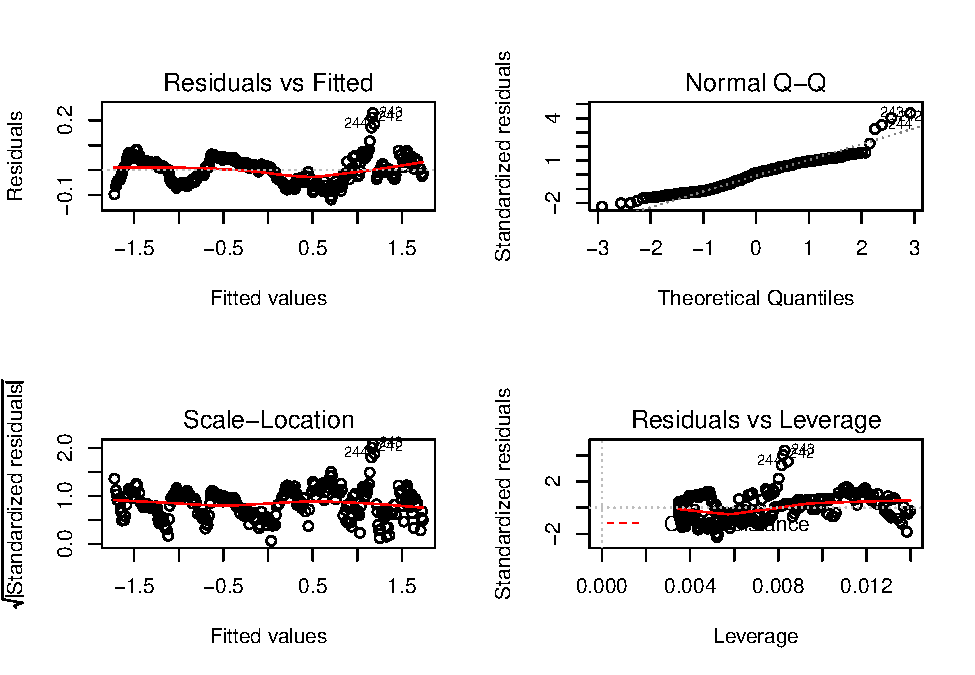
\includegraphics{HW1_files/figure-latex/unnamed-chunk-10-1.pdf}

Predictors such as TEAM\_FIELDING\_DP and TEAM\_FIELDING\_E do not
correlate well with a correlation value of around zero. Meanwhile, the
predictors TEAM\_BATTING\_HR and TEAM\_PITCHING\_HR have strong positive
correlations of nearly one. Functionally, this makes sense since the
quantity of pitches that gave a home run are directly effected by the
quantity of batters that hit home runs. For our purposes, we are mainly
concerned with the top row of correlations with game wins which are the
most important to our model.

If we want to make accurate predictions we need to include the the most
feasible predictors with correlations that have the strongest
relationships with the winnings. We understand that autocorrelated
predictors are impractical and will misrepresent the relationships
between predictors. In some other cases, the relationship may be strong
enough to use only one or two predictors for a model. For us, this is
not the case. Take a look at this table of correlations.

\begin{Shaded}
\begin{Highlighting}[]
\CommentTok{\# Gather complete observations}
\NormalTok{cors }\OtherTok{\textless{}{-}}\NormalTok{ tdata }\SpecialCharTok{\%\textgreater{}\%} 
  \FunctionTok{cor}\NormalTok{(., }\AttributeTok{use =} \StringTok{"complete.obs"}\NormalTok{) }
\CommentTok{\# Create fillable matrix}
\NormalTok{cors[}\FunctionTok{lower.tri}\NormalTok{(cors, }\AttributeTok{diag=}\ConstantTok{TRUE}\NormalTok{)] }\OtherTok{\textless{}{-}} \StringTok{""}
\CommentTok{\# Use observations to find correlation with wins}
\NormalTok{cors }\OtherTok{\textless{}{-}}\NormalTok{ cors }\SpecialCharTok{\%\textgreater{}\%}
  \FunctionTok{as.data.frame}\NormalTok{() }\SpecialCharTok{\%\textgreater{}\%}
  \FunctionTok{rownames\_to\_column}\NormalTok{() }\SpecialCharTok{\%\textgreater{}\%}
  \FunctionTok{gather}\NormalTok{(Variable, Correlation, }\SpecialCharTok{{-}}\NormalTok{rowname) }\SpecialCharTok{\%\textgreater{}\%}
  \FunctionTok{mutate}\NormalTok{(}\AttributeTok{Correlation =} \FunctionTok{as.numeric}\NormalTok{(Correlation)) }\SpecialCharTok{\%\textgreater{}\%}
\CommentTok{\# Format table to include Strength of correlations}
  \FunctionTok{rename}\NormalTok{(}\StringTok{\textasciigrave{}}\AttributeTok{ Wins}\StringTok{\textasciigrave{}} \OtherTok{=}\NormalTok{ rowname) }\SpecialCharTok{\%\textgreater{}\%}
  \FunctionTok{filter}\NormalTok{(Correlation }\SpecialCharTok{!=} \StringTok{""}\NormalTok{) }\SpecialCharTok{\%\textgreater{}\%}
  \FunctionTok{arrange}\NormalTok{(}\FunctionTok{desc}\NormalTok{(}\FunctionTok{abs}\NormalTok{(Correlation))) }\SpecialCharTok{\%\textgreater{}\%} 
  \FunctionTok{filter}\NormalTok{(}\StringTok{\textasciigrave{}}\AttributeTok{ Wins}\StringTok{\textasciigrave{}} \SpecialCharTok{==} \StringTok{"TARGET\_WINS"}\NormalTok{) }\SpecialCharTok{\%\textgreater{}\%} 
  \FunctionTok{mutate}\NormalTok{(}\AttributeTok{Strength =} \FunctionTok{abs}\NormalTok{(Correlation)) }
\CommentTok{\# Display table of correlations}
\FunctionTok{kbl}\NormalTok{(cors, }\AttributeTok{booktabs =}\NormalTok{ T, }\AttributeTok{caption =} \StringTok{"Predictor Correlations with Wins"}\NormalTok{) }\SpecialCharTok{\%\textgreater{}\%}
  \FunctionTok{kable\_styling}\NormalTok{(}\AttributeTok{latex\_options =} \FunctionTok{c}\NormalTok{(}\StringTok{"striped"}\NormalTok{, }\StringTok{"hold\_position"}\NormalTok{),}
                \AttributeTok{full\_width =}\NormalTok{ F) }\SpecialCharTok{\%\textgreater{}\%}
  \FunctionTok{footnote}\NormalTok{(}\FunctionTok{c}\NormalTok{(}\StringTok{"No correlation is higher than 0.48"}\NormalTok{))}
\end{Highlighting}
\end{Shaded}

\begin{table}[!h]

\caption{\label{tab:unnamed-chunk-11}Predictor Correlations with Wins}
\centering
\begin{tabular}[t]{llrr}
\toprule
 Wins & Variable & Correlation & Strength\\
\midrule
\cellcolor{gray!6}{TARGET\_WINS} & \cellcolor{gray!6}{TEAM\_PITCHING\_H} & \cellcolor{gray!6}{0.4712343} & \cellcolor{gray!6}{0.4712343}\\
TARGET\_WINS & TEAM\_BATTING\_H & 0.4699467 & 0.4699467\\
\cellcolor{gray!6}{TARGET\_WINS} & \cellcolor{gray!6}{TEAM\_BATTING\_BB} & \cellcolor{gray!6}{0.4686879} & \cellcolor{gray!6}{0.4686879}\\
TARGET\_WINS & TEAM\_PITCHING\_BB & 0.4683988 & 0.4683988\\
\cellcolor{gray!6}{TARGET\_WINS} & \cellcolor{gray!6}{TEAM\_PITCHING\_HR} & \cellcolor{gray!6}{0.4224668} & \cellcolor{gray!6}{0.4224668}\\
\addlinespace
TARGET\_WINS & TEAM\_BATTING\_HR & 0.4224168 & 0.4224168\\
\cellcolor{gray!6}{TARGET\_WINS} & \cellcolor{gray!6}{TEAM\_FIELDING\_E} & \cellcolor{gray!6}{-0.3866880} & \cellcolor{gray!6}{0.3866880}\\
TARGET\_WINS & TEAM\_BATTING\_2B & 0.3129840 & 0.3129840\\
\cellcolor{gray!6}{TARGET\_WINS} & \cellcolor{gray!6}{TEAM\_PITCHING\_SO} & \cellcolor{gray!6}{-0.2293648} & \cellcolor{gray!6}{0.2293648}\\
TARGET\_WINS & TEAM\_BATTING\_SO & -0.2288927 & 0.2288927\\
\addlinespace
\cellcolor{gray!6}{TARGET\_WINS} & \cellcolor{gray!6}{TEAM\_FIELDING\_DP} & \cellcolor{gray!6}{-0.1958660} & \cellcolor{gray!6}{0.1958660}\\
TARGET\_WINS & TEAM\_BASERUN\_CS & -0.1787560 & 0.1787560\\
\cellcolor{gray!6}{TARGET\_WINS} & \cellcolor{gray!6}{TEAM\_BATTING\_3B} & \cellcolor{gray!6}{-0.1243459} & \cellcolor{gray!6}{0.1243459}\\
TARGET\_WINS & TEAM\_BATTING\_HBP & 0.0735042 & 0.0735042\\
\cellcolor{gray!6}{TARGET\_WINS} & \cellcolor{gray!6}{TEAM\_BASERUN\_SB} & \cellcolor{gray!6}{0.0148364} & \cellcolor{gray!6}{0.0148364}\\
\bottomrule
\multicolumn{4}{l}{\rule{0pt}{1em}\textit{Note: }}\\
\multicolumn{4}{l}{\rule{0pt}{1em}No correlation is higher than 0.48}\\
\end{tabular}
\end{table}

No correlation has a strength greater than 0.48, as shown in the table
of predictor correlations with wins. This implies that there are other
variables that influence whether a team wins a game. Fortunately, this
was expected since baseball, although it has a theoretical advantage
with exceptional individuals, remains a team sport.

Based on the strength of the correlation the variables home runs, hits
on base, number of walks, and errors when fielding have the greatest
probability of being the best predictors in our model. They represent
the upper 50\% of our correlations with the target variable, games won.
By contrast, stolen bases, double plays, and strikeouts from either the
pitcher or batter, do not exert as much influence over game outcome.

As it stands, there is still a significant influence from outliers,
missing data points, and variables we may not need. These correlations
give us a good sense of where to begin in preparing the data for the
model. But before we settle on these predictors, there are a few other
considerations to make that may sway our model tremendously.

\hypertarget{model-considerations}{%
\subsubsection{Model Considerations}\label{model-considerations}}

Before we prepare the data for modeling, we consider the bigger picture
and how this model holds under the scope of baseball. There are plenty
of factors that might influence the predictive power of the model that
are not necessarily present in the charts but certainly present in
reality. We start by thinking critically about the timeline of the
sport.

Given such a large span of history, there have been many changes from
the beginning of this analysis to the present day. These changes may
cause a team's success to change, thereby lowering the overall accuracy
of these statistics as predictors.

As an example of this, consider the social factors that changed the
fabric of baseball and the MLB since the start of this data set in 1871.
There was racial segregation which did not end until 1964 and jim crow
laws thereafter. There were several major wars including two world wars,
the creation of new leagues that divided the players into separate
groups and players began to contractually obligate themselves to play
for teams as their main profession. Additionally, the rules have changed
over time, all continuously shaping a sport that was invented just 32
years prior to the start of this study.

These are not factors that we can control for in the model. Rather, it
is important to consider them since they may have great influence over
the results and prediction accuracy. To learn from the model we must
understand the level and scope of influence outside variables not
included in this data set may have on the model itself. Otherwise, we
cannot hope to improve it.

\hypertarget{data-preparation}{%
\subsection{Data Preparation}\label{data-preparation}}

\hypertarget{sample-set}{%
\subsubsection{Sample Set}\label{sample-set}}

Based on this data set we have options to choose from when deciding how
to best prepare and test the data. In this training data set, the full
set of performance statistics are given from 1871 to 2006. This implies
that the data could be used for training a model built solely on this
set alone with no other sources of data. For simplicity, that is what we
will do. This begins by taking a sample.

\begin{Shaded}
\begin{Highlighting}[]
\CommentTok{\# Take sample of tdata or }
\CommentTok{\# Use evaluation data to predict wins }
\FunctionTok{set.seed}\NormalTok{(}\DecValTok{0621}\NormalTok{)}
\NormalTok{edata }\OtherTok{\textless{}{-}} \FunctionTok{read.csv}\NormalTok{(}\StringTok{"https://raw.githubusercontent.com/palmorezm/data621/main/moneyball{-}evaluation{-}data.csv"}\NormalTok{)}
\NormalTok{tsample\_300 }\OtherTok{\textless{}{-}} \FunctionTok{sample\_n}\NormalTok{(tdata[}\DecValTok{2}\SpecialCharTok{:}\DecValTok{17}\NormalTok{], }\DecValTok{300}\NormalTok{, }\AttributeTok{replace =} \ConstantTok{FALSE}\NormalTok{, }\AttributeTok{weight =} \ConstantTok{NULL}\NormalTok{) }\CommentTok{\# random sample of 300 rows; no replacement}
\NormalTok{edata }\OtherTok{\textless{}{-}}\NormalTok{ tsample\_300 }\CommentTok{\# will be used to predict win from random sample}
\end{Highlighting}
\end{Shaded}

The sample contains 300 randomly selected records from the training data
without replacement. For now, this data is stored as our evaluation
data. The first portion of the data set is shown for reference.

\begin{Shaded}
\begin{Highlighting}[]
\FunctionTok{head}\NormalTok{(edata) }\CommentTok{\# only 15 columns {-} index and games won are not included}
\end{Highlighting}
\end{Shaded}

\begin{verbatim}
##   TARGET_WINS TEAM_BATTING_H TEAM_BATTING_2B TEAM_BATTING_3B TEAM_BATTING_HR
## 1          75           1314             196              79              18
## 2          56           1435             205              55              26
## 3          74           1492             296              27             189
## 4          44           1533             221              79              25
## 5         100           1545             232              65             209
## 6          75           1437             218              80              38
##   TEAM_BATTING_BB TEAM_BATTING_SO TEAM_BASERUN_SB TEAM_BASERUN_CS
## 1             448             914             247             200
## 2             375             478              78              72
## 3             447             902              83              37
## 4             664             450             196              NA
## 5             485             767              37              17
## 6             504             697             265              NA
##   TEAM_BATTING_HBP TEAM_PITCHING_H TEAM_PITCHING_HR TEAM_PITCHING_BB
## 1               NA            1391               19              474
## 2               NA            1519               28              397
## 3               54            1492              189              447
## 4               NA            1881               31              815
## 5               NA            1625              220              510
## 6               NA            1532               41              537
##   TEAM_PITCHING_SO TEAM_FIELDING_E TEAM_FIELDING_DP
## 1              968             336              121
## 2              506             178              163
## 3              902             107              154
## 4              552             603               NA
## 5              807             126              182
## 6              743             304              110
\end{verbatim}

Later in the analysis, we will use this test evaluation data (or edata),
to test the selected model since it is quite similar to our training
data (but not exactly the same). This too can be shown. Observe the
differences in missing data from the sample and training data sets.

\begin{Shaded}
\begin{Highlighting}[]
\CommentTok{\# calculate missing values}
\NormalTok{edata.missing.values }\OtherTok{\textless{}{-}} \FunctionTok{sum}\NormalTok{(}\FunctionTok{is.na}\NormalTok{(edata))}
\NormalTok{edata.total.obs }\OtherTok{\textless{}{-}} \FunctionTok{count}\NormalTok{(edata)}
\CommentTok{\# find number of fields}
\NormalTok{edata.fields }\OtherTok{\textless{}{-}} \FunctionTok{ncol}\NormalTok{(edata)}
\NormalTok{tdata.fields }\OtherTok{\textless{}{-}} \FunctionTok{ncol}\NormalTok{(tdata)}
\CommentTok{\# find total entries }
\NormalTok{edata.entry }\OtherTok{\textless{}{-}}\NormalTok{ edata.total.obs }\SpecialCharTok{*} \FunctionTok{ncol}\NormalTok{(edata)}
\NormalTok{tdata.entry }\OtherTok{\textless{}{-}}\NormalTok{ total.obs }\SpecialCharTok{*} \FunctionTok{ncol}\NormalTok{(tdata)}
\CommentTok{\# calculate percent missing}
\NormalTok{edata.percent.missing }\OtherTok{\textless{}{-}}\NormalTok{ edata.missing.values }\SpecialCharTok{/}\NormalTok{ edata.entry }\SpecialCharTok{*} \DecValTok{100}
\NormalTok{percent.missing }\OtherTok{\textless{}{-}}\NormalTok{ missing.values }\SpecialCharTok{/}\NormalTok{ tdata.entry }\SpecialCharTok{*} \DecValTok{100}

\CommentTok{\# create matrix of values}
\NormalTok{compare.data }\OtherTok{\textless{}{-}} \FunctionTok{matrix}\NormalTok{(}\FunctionTok{c}\NormalTok{(edata.missing.values, }
\NormalTok{                         missing.values, }
\NormalTok{                         edata.total.obs, }
\NormalTok{                         total.obs, }
\NormalTok{                         tdata.fields, }
\NormalTok{                         edata.fields, }
\NormalTok{                         edata.entry, }
\NormalTok{                         tdata.entry,}
                         \FunctionTok{round}\NormalTok{(edata.percent.missing, }\AttributeTok{digits=}\DecValTok{2}\NormalTok{), }
                         \FunctionTok{round}\NormalTok{(percent.missing, }\AttributeTok{digits=}\DecValTok{2}\NormalTok{)), }\AttributeTok{ncol=}\DecValTok{5}\NormalTok{, }\AttributeTok{byrow=}\ConstantTok{FALSE}\NormalTok{)}
\NormalTok{compare.data}
\end{Highlighting}
\end{Shaded}

\begin{verbatim}
##      [,1] [,2] [,3] [,4]  [,5]
## [1,] 463  300  17   4800  9.65
## [2,] 3478 2276 16   38692 8.99
\end{verbatim}

\begin{Shaded}
\begin{Highlighting}[]
\NormalTok{compare.data }\OtherTok{\textless{}{-}} \FunctionTok{as.data.frame}\NormalTok{(compare.data)}
\NormalTok{header }\OtherTok{\textless{}{-}} \FunctionTok{c}\NormalTok{(}\StringTok{"Missing Values"}\NormalTok{, }\StringTok{"Observations"}\NormalTok{, }\StringTok{"Fields"}\NormalTok{, }\StringTok{"Total Entries"}\NormalTok{, }\StringTok{"Percent Missing"}\NormalTok{)}
\NormalTok{row }\OtherTok{\textless{}{-}} \FunctionTok{c}\NormalTok{(}\StringTok{"eData"}\NormalTok{, }\StringTok{"tData"}\NormalTok{)}
\FunctionTok{colnames}\NormalTok{(compare.data) }\OtherTok{\textless{}{-}}\NormalTok{ header}
\FunctionTok{row.names}\NormalTok{(compare.data) }\OtherTok{\textless{}{-}}\NormalTok{ row }
\FunctionTok{kbl}\NormalTok{(compare.data)}
\end{Highlighting}
\end{Shaded}

\begin{tabular}[t]{l|l|l|l|l|l}
\hline
  & Missing Values & Observations & Fields & Total Entries & Percent Missing\\
\hline
eData & 463 & 300 & 17 & 4800 & 9.65\\
\hline
tData & 3478 & 2276 & 16 & 38692 & 8.99\\
\hline
\end{tabular}

The training and sample data have relatively similar missing data
points. One might expect that if the data were randomly sampled from the
training data set then the relationships between the variables should be
largely preserved. We rely on these principles in future testing.

\hypertarget{adjustments}{%
\subsubsection{Adjustments}\label{adjustments}}

When we explored the data set we found that there were missing values in
the data. These should be fixed or removed. We also discovered that some
fields were impractical or had little to no influence over prediction.
These fields should also be removed. Outliers are also a major concern
and must be dealt with. Additionally, we fix the remaining missing
values by assigning them the median value of the distribution so as to
prevent altering the relationship too much. Performing these adjustments
should improve the model.

\begin{Shaded}
\begin{Highlighting}[]
\CommentTok{\# select all but index, batting\_hbp, baserun\_cs}
\CommentTok{\# replace missing values with the median value for the distribution}
\NormalTok{tdata }\OtherTok{\textless{}{-}}\NormalTok{ tdata }\SpecialCharTok{\%\textgreater{}\%}
  \FunctionTok{rename}\NormalTok{(}\StringTok{"win"} \OtherTok{=}\NormalTok{TARGET\_WINS, }\CommentTok{\# For use with edata sampling}
        \StringTok{"bhit"} \OtherTok{=}\NormalTok{TEAM\_BATTING\_H, }
        \StringTok{"bdouble"}  \OtherTok{=}\NormalTok{ TEAM\_BATTING\_2B, }
        \StringTok{"btriple"}  \OtherTok{=}\NormalTok{ TEAM\_BATTING\_3B, }
        \StringTok{"bhomerun"}  \OtherTok{=}\NormalTok{ TEAM\_BATTING\_HR, }
        \StringTok{"bwalk"}  \OtherTok{=}\NormalTok{ TEAM\_BATTING\_BB, }
        \StringTok{"bstrikeout"}  \OtherTok{=}\NormalTok{ TEAM\_BATTING\_SO, }
        \StringTok{"stolenbase"}  \OtherTok{=}\NormalTok{ TEAM\_BASERUN\_SB, }
        \StringTok{"caught"}  \OtherTok{=}\NormalTok{ TEAM\_BASERUN\_CS, }
        \StringTok{"bhitbyp"}  \OtherTok{=}\NormalTok{ TEAM\_BATTING\_HBP, }
        \StringTok{"phit"}  \OtherTok{=}\NormalTok{ TEAM\_PITCHING\_H, }
        \StringTok{"phomerun"}  \OtherTok{=}\NormalTok{ TEAM\_PITCHING\_HR, }
        \StringTok{"pwalk"}  \OtherTok{=}\NormalTok{ TEAM\_PITCHING\_BB, }
        \StringTok{"pstrikeout"}  \OtherTok{=}\NormalTok{ TEAM\_PITCHING\_SO, }
        \StringTok{"fielderror"}  \OtherTok{=}\NormalTok{ TEAM\_FIELDING\_E, }
        \StringTok{"fielddp"}  \OtherTok{=}\NormalTok{ TEAM\_FIELDING\_DP) }
\end{Highlighting}
\end{Shaded}

\begin{Shaded}
\begin{Highlighting}[]
\CommentTok{\# drops insignificant columns }
\CommentTok{\# replaces NA with median (given a removal of missing values in calculation)}
\NormalTok{df }\OtherTok{\textless{}{-}}\NormalTok{ tdata[}\FunctionTok{c}\NormalTok{(}\DecValTok{2}\SpecialCharTok{:}\DecValTok{9}\NormalTok{,}\DecValTok{12}\SpecialCharTok{:}\DecValTok{17}\NormalTok{)]          }\CommentTok{\# use if raw tdata}
\CommentTok{\# df \textless{}{-} tdata[c(1:7,10:15)] \# use with sampled tdata excluding win variable}
\CommentTok{\# produces 13 columns/fields with sampled tdata excluding win variable}
\CommentTok{\# produces 15 columns/fields with raw tdata excluding win variable}
\ControlFlowTok{for}\NormalTok{ (i }\ControlFlowTok{in} \FunctionTok{colnames}\NormalTok{(df)) \{}
\NormalTok{  df[[i]][}\FunctionTok{is.na}\NormalTok{(df[[i]])] }\OtherTok{\textless{}{-}} \FunctionTok{median}\NormalTok{(df[[i]], }\AttributeTok{na.rm=}\ConstantTok{TRUE}\NormalTok{)}
\NormalTok{\}}
\end{Highlighting}
\end{Shaded}

Above, we convert the field variable name into something readable and
easier to work with. Then insignificant fields are removed. The
selection process is based on those variables that had low correlations
near zero, in the exploration section. Missing values are then replaced
with the median value for the distribution. Importantly, this
calculation was made assuming there were no missing values so as not to
further skew or deviate from the original distribution. The median was
chosen due to its status as a robust statistic.

Next, we identify and remove outliers. As shown in the violin plots with
box plots overlaid, there are quite a few extreme data points that are
skewing many variables. Some of these have high correlation values and
may make for good predictors. These are dealt with using the
interquartile range (IQR) of each field's distribution.

\begin{Shaded}
\begin{Highlighting}[]
\CommentTok{\# remove outliers based on IQR}
\ControlFlowTok{for}\NormalTok{ (i }\ControlFlowTok{in} \FunctionTok{colnames}\NormalTok{(df)) \{}
\NormalTok{  iqr }\OtherTok{\textless{}{-}} \FunctionTok{IQR}\NormalTok{(df[[i]])}
\NormalTok{  q }\OtherTok{\textless{}{-}} \FunctionTok{quantile}\NormalTok{(df[[i]], }\AttributeTok{probs =} \FunctionTok{c}\NormalTok{(}\FloatTok{0.25}\NormalTok{, }\FloatTok{0.75}\NormalTok{), }\AttributeTok{na.rm =} \ConstantTok{FALSE}\NormalTok{)}
\NormalTok{  qupper }\OtherTok{\textless{}{-}}\NormalTok{ q[}\DecValTok{2}\NormalTok{]}\SpecialCharTok{+}\FloatTok{1.5}\SpecialCharTok{*}\NormalTok{iqr}
\NormalTok{  qlower }\OtherTok{\textless{}{-}}\NormalTok{ q[}\DecValTok{1}\NormalTok{]}\SpecialCharTok{+}\FloatTok{1.5}\SpecialCharTok{*}\NormalTok{iqr}
\NormalTok{  outlier\_free }\OtherTok{\textless{}{-}} \FunctionTok{subset}\NormalTok{(df, df[[i]] }\SpecialCharTok{\textgreater{}}\NormalTok{ (q[}\DecValTok{1}\NormalTok{] }\SpecialCharTok{{-}} \FloatTok{1.5}\SpecialCharTok{*}\NormalTok{iqr) }\SpecialCharTok{\&}\NormalTok{ df[[i]] }\SpecialCharTok{\textless{}}\NormalTok{ (q[}\DecValTok{2}\NormalTok{]}\SpecialCharTok{+}\FloatTok{1.5}\SpecialCharTok{*}\NormalTok{iqr) )}
\NormalTok{\}}
\NormalTok{df }\OtherTok{\textless{}{-}}\NormalTok{ outlier\_free}
\end{Highlighting}
\end{Shaded}

Cycling through each variable in the data, where outliers are found the
data is subset, effectively removing the data points from each field.
Outliers were determined by one standard deviation above the upper and
below the lower quartile in each distribution. This gave us a little bit
of wiggle room to include rare occurrences but exclude extreme values.
Given a bit of domain knowledge, some outlier points are possible while
others are not which means a small amount of these outliers will remain,
as they should, in each field.

\hypertarget{new-estimates}{%
\subsubsection{New Estimates}\label{new-estimates}}

Based on the descriptions of the available fields, there are no singles
from batters. While this is theoretically possible, in reality, the
probability of there never being a single base hit in baseball for the
MLB is near impossible. This is corrected and an additional field, one
that we are calling `gt1base' is computed as new field estimates.

\begin{Shaded}
\begin{Highlighting}[]
\CommentTok{\# Create new estimates from stats}
\NormalTok{df }\OtherTok{\textless{}{-}}\NormalTok{ df }\SpecialCharTok{\%\textgreater{}\%} 
  \CommentTok{\# Hits resulting in greater than one base }
  \FunctionTok{mutate}\NormalTok{(}\AttributeTok{gt1base =}\NormalTok{ bdouble }\SpecialCharTok{+}\NormalTok{ btriple }\SpecialCharTok{+}\NormalTok{ bhomerun) }\SpecialCharTok{\%\textgreater{}\%} 
  \CommentTok{\# Hits resulting in one base}
  \FunctionTok{mutate}\NormalTok{(}\AttributeTok{bsingle =}\NormalTok{ bhit }\SpecialCharTok{{-}}\NormalTok{ gt1base)}
\end{Highlighting}
\end{Shaded}

We created the `gt1base' from the sum of performance statistics about
base hits. As its name implies, it records base hits that are greater
than one base. That is, all doubles, triples, and homeruns. This may
help prove that big hitters improve the outcome of games.

Singles from batters are also created as a new estimate. Specifically,
this records the number of batters that hit the ball and got to first
base. To get singles, we found the difference in total hits from those
with `gt1base'. As with `gt1base', these new estimates are calculated
based on the year they were recorded.

\hypertarget{predictor-ratios}{%
\subsubsection{Predictor Ratios}\label{predictor-ratios}}

When exploring, the strongest correlations, or specifically, those that
were in the upper half of the correlation table, had autocorrelations
that resulted in strength values near one. Rather than have to drop the
strength of these correlations, it might prove beneficial to the model
if we can leverage the strength of these correlations as a ratio. Thus,
they were computed.

\begin{Shaded}
\begin{Highlighting}[]
\CommentTok{\# Compute predictor ratios}
\NormalTok{df }\OtherTok{\textless{}{-}}\NormalTok{ df }\SpecialCharTok{\%\textgreater{}\%} 
  \FunctionTok{mutate}\NormalTok{(}\AttributeTok{pbh =}\NormalTok{ phit}\SpecialCharTok{/}\NormalTok{bhit) }\SpecialCharTok{\%\textgreater{}\%} 
  \FunctionTok{mutate}\NormalTok{(}\AttributeTok{pbhr =}\NormalTok{ phomerun}\SpecialCharTok{/}\NormalTok{bhomerun) }\SpecialCharTok{\%\textgreater{}\%} 
  \FunctionTok{mutate}\NormalTok{(}\AttributeTok{pbw =}\NormalTok{ pwalk}\SpecialCharTok{/}\NormalTok{bwalk) }\SpecialCharTok{\%\textgreater{}\%} 
  \FunctionTok{mutate}\NormalTok{(}\AttributeTok{fdpe =}\NormalTok{ fielddp}\SpecialCharTok{/}\NormalTok{fielderror)}
\end{Highlighting}
\end{Shaded}

Hits from batters thrown by pitchers, for example, is not an independent
relationship. The pitcher must throw for the batter to hit and unless
the pitcher intentionally allows the batter to hit the ball, then they
are in fact directly caused by one another. To make use of it, the ratio
of times the pitcher threw the ball to the number of times the batter
hit the ball, is a valid, independent event (or rather series of events)
that may lead to a better outcome and increase the chances of a team to
win a game. The remaining ratios follow this same principle.

We calculated how many times a pitcher allowed a homerun with the number
of times the batter hit a homerun. The number of times the pitcher gave
the batter a walk and the number of times the batter walked. Lastly, the
number of times fielders made a double play compared to the number of
times fielders made a mistake.

\hypertarget{transformations}{%
\subsubsection{Transformations}\label{transformations}}

At this point, some of the data remains abnormal. Those distributions in
the exploratory section describe how TEAM\_FIELDING\_E,
TEAM\_PITCHING\_BB, TEAM\_PITCHING\_H, and TEAM\_PITCHING\_SO exhibit
non-normal, perhaps nonlinear trends. To fix this we need to determine
what the best kind of transformation is to normalize it. We do so using
the bestNormalize function within the `bestNormalize' package. The
process is shown.

\begin{Shaded}
\begin{Highlighting}[]
\CommentTok{\# determine best way to transform and their metrics}
\NormalTok{bestNorms }\OtherTok{\textless{}{-}}\NormalTok{ df[}\DecValTok{1}\SpecialCharTok{:}\DecValTok{11}\NormalTok{,]}
\ControlFlowTok{for}\NormalTok{ (i }\ControlFlowTok{in} \FunctionTok{colnames}\NormalTok{(df)) \{}
\NormalTok{  bestNorms[[i]] }\OtherTok{\textless{}{-}} \FunctionTok{bestNormalize}\NormalTok{(df[[i]], }\AttributeTok{allow\_orderNorm =} \ConstantTok{FALSE}\NormalTok{, }\AttributeTok{out\_of\_sample =} \ConstantTok{FALSE}\NormalTok{)}
\NormalTok{\}}
\end{Highlighting}
\end{Shaded}

In this function, it performs multiple normalizing transformations
including the Lambert W x F, Box-Cox, Yeo-Johnson, transformations along
with other methods like the ordered quantile technique. The results are
then reviewed by the function to determine which distribution and
associated residuals appear the most Gausian. It relies on a few other
functions, like those of the MASS package, to estimate the best value of
lambda or other appropriate variables necessary for performing the
transformation and produces a list of recommendations.

\begin{Shaded}
\begin{Highlighting}[]
\CommentTok{\# focus on problem areas; those with non{-}normal stats}
\NormalTok{bestNorms}\SpecialCharTok{$}\NormalTok{fielderror}\SpecialCharTok{$}\NormalTok{chosen\_transform}
\end{Highlighting}
\end{Shaded}

\begin{verbatim}
## Standardized Yeo-Johnson Transformation with 2184 nonmissing obs.:
##  Estimated statistics:
##  - lambda = -0.9878936 
##  - mean (before standardization) = 1.005778 
##  - sd (before standardization) = 0.002801129
\end{verbatim}

\begin{Shaded}
\begin{Highlighting}[]
\NormalTok{bestNorms}\SpecialCharTok{$}\NormalTok{pwalk}\SpecialCharTok{$}\NormalTok{chosen\_transform}
\end{Highlighting}
\end{Shaded}

\begin{verbatim}
## Standardized Yeo-Johnson Transformation with 2184 nonmissing obs.:
##  Estimated statistics:
##  - lambda = 0.301843 
##  - mean (before standardization) = 18.87912 
##  - sd (before standardization) = 1.68402
\end{verbatim}

\begin{Shaded}
\begin{Highlighting}[]
\NormalTok{bestNorms}\SpecialCharTok{$}\NormalTok{phit}\SpecialCharTok{$}\NormalTok{chosen\_transform}
\end{Highlighting}
\end{Shaded}

\begin{verbatim}
## Standardized Yeo-Johnson Transformation with 2184 nonmissing obs.:
##  Estimated statistics:
##  - lambda = -3.125283 
##  - mean (before standardization) = 0.319971 
##  - sd (before standardization) = 1.435836e-11
\end{verbatim}

\begin{Shaded}
\begin{Highlighting}[]
\NormalTok{bestNorms}\SpecialCharTok{$}\NormalTok{pstrikeout}\SpecialCharTok{$}\NormalTok{chosen\_transform}
\end{Highlighting}
\end{Shaded}

\begin{verbatim}
## Standardized Yeo-Johnson Transformation with 2184 nonmissing obs.:
##  Estimated statistics:
##  - lambda = 0.4299074 
##  - mean (before standardization) = 38.4267 
##  - sd (before standardization) = 7.402144
\end{verbatim}

The Yeo-Johnson is the preferred choice given the options available in
the bestNormalize function. Perhaps, unsurprisingly, since these
distributions shared the same levels of skew, nonlinearity, and
heteroscedasticity, the same transformation is recommended for each.
This is similar to a Box-Cox transformation but can work on a wider
array of values. An example Yeo-Johnson is performed below with
associate box plots and histograms for reference.

\begin{Shaded}
\begin{Highlighting}[]
\CommentTok{\# Example Yeo{-}Johnson transformation }
\NormalTok{test }\OtherTok{\textless{}{-}}\NormalTok{ df}
\NormalTok{test}\SpecialCharTok{$}\NormalTok{fielderror }\OtherTok{\textless{}{-}} \FunctionTok{yeo.johnson}\NormalTok{(df}\SpecialCharTok{$}\NormalTok{fielderror, }\AttributeTok{lambda =} \SpecialCharTok{{-}}\FloatTok{0.9878936}\NormalTok{, }\AttributeTok{derivative =} \DecValTok{0}\NormalTok{, }\AttributeTok{epsilon =} \FunctionTok{sqrt}\NormalTok{(.Machine}\SpecialCharTok{$}\NormalTok{double.eps), }\AttributeTok{inverse =} \ConstantTok{FALSE}\NormalTok{)}
\FunctionTok{boxplot}\NormalTok{(test}\SpecialCharTok{$}\NormalTok{fielderror, }\AttributeTok{main=} \StringTok{"Tranformed Field Error Box plot"}\NormalTok{)}
\end{Highlighting}
\end{Shaded}

\includegraphics{HW1_files/figure-latex/unnamed-chunk-22-1.pdf}

\begin{Shaded}
\begin{Highlighting}[]
\FunctionTok{hist}\NormalTok{(test}\SpecialCharTok{$}\NormalTok{fielderror, }\AttributeTok{main=} \StringTok{"Tranformed Field Error Distriubtion"}\NormalTok{)}
\end{Highlighting}
\end{Shaded}

\includegraphics{HW1_files/figure-latex/unnamed-chunk-22-2.pdf}

\begin{Shaded}
\begin{Highlighting}[]
\FunctionTok{boxplot}\NormalTok{(df}\SpecialCharTok{$}\NormalTok{fielderror, }\AttributeTok{main=} \StringTok{"Original Field Error Box plot"}\NormalTok{)}
\end{Highlighting}
\end{Shaded}

\includegraphics{HW1_files/figure-latex/unnamed-chunk-22-3.pdf}

\begin{Shaded}
\begin{Highlighting}[]
\FunctionTok{hist}\NormalTok{(df}\SpecialCharTok{$}\NormalTok{fielderror, }\AttributeTok{main=} \StringTok{"Original Field Error Box plot"}\NormalTok{)}
\end{Highlighting}
\end{Shaded}

\includegraphics{HW1_files/figure-latex/unnamed-chunk-22-4.pdf}

Notice how the distribution normalizes from a large right skew to a
nearly perfectly normal distribution. The box plot distribution also
shows that there are far fewer outliers since our attempt to limit them.
Our transformation appears to have also assisted with the reduction of
those extreme values, as well as normalizing. The Yeo-Johnson
transformation is applied to the other variables in the same way with
their appropriate values of lambda.

\begin{Shaded}
\begin{Highlighting}[]
\CommentTok{\# Applying Yeo{-}Johnson transformation}
\NormalTok{df}\SpecialCharTok{$}\NormalTok{fielderror }\OtherTok{\textless{}{-}} \FunctionTok{yeo.johnson}\NormalTok{(df}\SpecialCharTok{$}\NormalTok{fielderror, }\AttributeTok{lambda =} \SpecialCharTok{{-}}\FloatTok{0.9878936}\NormalTok{, }\AttributeTok{derivative =} \DecValTok{0}\NormalTok{, }\AttributeTok{epsilon =} \FunctionTok{sqrt}\NormalTok{(.Machine}\SpecialCharTok{$}\NormalTok{double.eps), }\AttributeTok{inverse =} \ConstantTok{FALSE}\NormalTok{)}
\NormalTok{df}\SpecialCharTok{$}\NormalTok{pwalk }\OtherTok{\textless{}{-}} \FunctionTok{yeo.johnson}\NormalTok{(df}\SpecialCharTok{$}\NormalTok{pwalk, }\AttributeTok{lambda =} \FloatTok{0.301843}\NormalTok{, }\AttributeTok{derivative =} \DecValTok{0}\NormalTok{, }\AttributeTok{epsilon =} \FunctionTok{sqrt}\NormalTok{(.Machine}\SpecialCharTok{$}\NormalTok{double.eps), }\AttributeTok{inverse =} \ConstantTok{FALSE}\NormalTok{)}
\NormalTok{df}\SpecialCharTok{$}\NormalTok{phit }\OtherTok{\textless{}{-}} \FunctionTok{yeo.johnson}\NormalTok{(df}\SpecialCharTok{$}\NormalTok{phit, }\AttributeTok{lambda =} \SpecialCharTok{{-}}\FloatTok{3.125283}\NormalTok{, }\AttributeTok{derivative =} \DecValTok{0}\NormalTok{, }\AttributeTok{epsilon =} \FunctionTok{sqrt}\NormalTok{(.Machine}\SpecialCharTok{$}\NormalTok{double.eps), }\AttributeTok{inverse =} \ConstantTok{FALSE}\NormalTok{)}
\NormalTok{df}\SpecialCharTok{$}\NormalTok{pstrikeout }\OtherTok{\textless{}{-}} \FunctionTok{yeo.johnson}\NormalTok{(df}\SpecialCharTok{$}\NormalTok{pstrikeout, }\AttributeTok{lambda =} \FloatTok{0.4299074}\NormalTok{, }\AttributeTok{derivative =} \DecValTok{0}\NormalTok{, }\AttributeTok{epsilon =} \FunctionTok{sqrt}\NormalTok{(.Machine}\SpecialCharTok{$}\NormalTok{double.eps), }\AttributeTok{inverse =} \ConstantTok{FALSE}\NormalTok{)}
\end{Highlighting}
\end{Shaded}

We re-evaluate for missing or non-applicable data points to ensure none
remain. We should not have any for our original variables but the new
estimates we created need adjusting. The same process for fixing missing
values is applied. A new median metric is found for each estimate and
stored in place of the missing value thereby limiting the change to the
distribution or relationship between variables.

\begin{Shaded}
\begin{Highlighting}[]
\CommentTok{\# Reassign median values to new ratios where NA value is present}
\ControlFlowTok{for}\NormalTok{ (i }\ControlFlowTok{in} \FunctionTok{colnames}\NormalTok{(df)) \{}
\NormalTok{  df[[i]][}\FunctionTok{is.na}\NormalTok{(df[[i]])] }\OtherTok{\textless{}{-}} \FunctionTok{median}\NormalTok{(df[[i]], }\AttributeTok{na.rm=}\ConstantTok{TRUE}\NormalTok{)}
\NormalTok{\}}
\CommentTok{\# sum(is.na(df)) \# ensure no missing values remain}
\end{Highlighting}
\end{Shaded}

\hypertarget{review}{%
\subsubsection{Review}\label{review}}

\begin{Shaded}
\begin{Highlighting}[]
\CommentTok{\# New variables}
\FunctionTok{head}\NormalTok{(df[}\DecValTok{15}\SpecialCharTok{:}\DecValTok{20}\NormalTok{]) }\CommentTok{\# raw tdata only}
\end{Highlighting}
\end{Shaded}

\begin{verbatim}
##   gt1base bsingle      pbh     pbhr      pbw      fdpe
## 1     246    1199 6.480277 6.461538 6.482517 0.1473788
## 2     431     908 1.005975 1.005263 1.005839 0.8031088
## 3     404     973 1.000000 1.000000 1.000000 0.8742857
## 4     343    1044 1.006489 1.010417 1.006652 0.9512195
## 5     315     982 1.000000 1.000000 1.000000 1.2173913
## 6     328     951 1.000000 1.000000 1.000000 1.2113821
\end{verbatim}

\begin{Shaded}
\begin{Highlighting}[]
\CommentTok{\# head(df[14:19]) \# sample edata only}
\end{Highlighting}
\end{Shaded}

\begin{Shaded}
\begin{Highlighting}[]
\FunctionTok{head}\NormalTok{(df[}\DecValTok{1}\SpecialCharTok{:}\DecValTok{14}\NormalTok{]) }\CommentTok{\# raw tdata only}
\end{Highlighting}
\end{Shaded}

\begin{verbatim}
##   win bhit bdouble btriple bhomerun bwalk bstrikeout stolenbase     phit
## 1  39 1445     194      39       13   143        842        101 0.319971
## 2  70 1339     219      22      190   685       1075         37 0.319971
## 3  86 1377     232      35      137   602        917         46 0.319971
## 4  70 1387     209      38       96   451        922         43 0.319971
## 5  82 1297     186      27      102   472        920         49 0.319971
## 6  75 1279     200      36       92   443        973        107 0.319971
##   phomerun    pwalk pstrikeout fielderror fielddp
## 1       84 22.74570   91.68288   1.011167     149
## 2      191 20.51601   44.58056   1.006693     155
## 3      137 19.56608   41.36302   1.006132     153
## 4       97 17.70161   41.58731   1.005729     156
## 5      102 17.94916   41.42434   1.004524     168
## 6       92 17.54695   42.48946   1.003601     149
\end{verbatim}

\begin{Shaded}
\begin{Highlighting}[]
\CommentTok{\# head(df[1:13]) \# sample edata only}
\end{Highlighting}
\end{Shaded}

\hypertarget{model-building}{%
\subsection{Model Building}\label{model-building}}

\hypertarget{types}{%
\subsubsection{Types}\label{types}}

There are many kinds of models that could be used to predict this data.
However, the best model is not clear. To determine which models are best
we will assess the training data through multiple models and compare.
Those models include a kitchen sink approach, high correlations model,
ratio model, and a polynomial model with a twist. We refrain from
ensemble modeling to avoid overcomplicating and accidentally introducing
errors in the prediction.

\hypertarget{reasoning}{%
\subsubsection{Reasoning}\label{reasoning}}

Our first choice of model is the kitchen sink. This was chosen because
it can act as a sort of preliminary test to see what patterns arise when
we pass all the variables through it. As the saying goes, we are
throwing everything but the kitchen sink at it to see what works. This
should help inform our choices for the remaining models.

Our second and third models are the high correlation and ratio models.
High correlation model is just that, a model with only the top 50\% of
variables that correlated better than the other variables with the
target variable wins. The ratio model follows the same principle by
taking the computed ratios and assessing how well they predict the
target. We do not expect either of these models to produce better
results than the kitchen sink model due to the nature of the predictors,
most notably that correlation does not equate to causation. However,
they will help inform us of the outcome if one judged the likelihood of
games by their most phenomenal characteristics.

Last is the polynomial model, but with a twist. We are going to raise
the order of the polynomial sequentially from the first to the third
degree then instead of running the model altogether, tell it to pick the
variables that result in the highest coefficients of determination. The
twist here is in the selection process for the polynomial. Since it is
run forwards and backwards to determine the best fit, this should be a
good choice for prediction if there is indeed a linear relationship
present.

\hypertarget{creation}{%
\subsubsection{Creation}\label{creation}}

The first model is created following the kitchen sink method. Subsequent
aforementioned models are run thereafter. A summary of the results is
displayed below each model containing the errors for each predictor,
residual summaries, respective coefficients of determination, p-values
and more. An analysis of these is to follow.

\begin{Shaded}
\begin{Highlighting}[]
\CommentTok{\# Kitchen sink}
\NormalTok{model.ks }\OtherTok{\textless{}{-}} \FunctionTok{lm}\NormalTok{(win}\SpecialCharTok{\textasciitilde{}}\NormalTok{., df)}
\FunctionTok{summary}\NormalTok{(model.ks)}
\end{Highlighting}
\end{Shaded}

\begin{verbatim}
## 
## Call:
## lm(formula = win ~ ., data = df)
## 
## Residuals:
##     Min      1Q  Median      3Q     Max 
## -51.966  -8.055  -0.016   8.039  66.645 
## 
## Coefficients: (3 not defined because of singularities)
##               Estimate Std. Error t value Pr(>|t|)    
## (Intercept) 116.628153 857.859972   0.136 0.891872    
## bhit          0.044995   0.003850  11.688  < 2e-16 ***
## bdouble      -0.026595   0.009422  -2.823 0.004807 ** 
## btriple       0.096432   0.017548   5.495 4.36e-08 ***
## bhomerun      0.012773   0.032299   0.395 0.692547    
## bwalk         0.030271   0.008345   3.628 0.000293 ***
## bstrikeout   -0.021044   0.003637  -5.787 8.23e-09 ***
## stolenbase    0.027267   0.004195   6.499 9.99e-11 ***
## phit                NA         NA      NA       NA    
## phomerun      0.037582   0.028790   1.305 0.191900    
## pwalk        -1.172939   0.566361  -2.071 0.038476 *  
## pstrikeout    0.480884   0.093710   5.132 3.13e-07 ***
## fielderror  -82.889511 852.282744  -0.097 0.922532    
## fielddp      -0.208871   0.037336  -5.594 2.49e-08 ***
## gt1base             NA         NA      NA       NA    
## bsingle             NA         NA      NA       NA    
## pbh          -1.377182   0.552550  -2.492 0.012762 *  
## pbhr         -1.958194   1.048096  -1.868 0.061850 .  
## pbw           0.015477   0.895341   0.017 0.986210    
## fdpe         13.726684   5.805135   2.365 0.018138 *  
## ---
## Signif. codes:  0 '***' 0.001 '**' 0.01 '*' 0.05 '.' 0.1 ' ' 1
## 
## Residual standard error: 12.8 on 2167 degrees of freedom
## Multiple R-squared:   0.33,  Adjusted R-squared:  0.325 
## F-statistic:  66.7 on 16 and 2167 DF,  p-value: < 2.2e-16
\end{verbatim}

\begin{Shaded}
\begin{Highlighting}[]
\CommentTok{\# High correlations model}
\NormalTok{model.hc }\OtherTok{\textless{}{-}} \FunctionTok{lm}\NormalTok{(win}\SpecialCharTok{\textasciitilde{}}\NormalTok{ phit }\SpecialCharTok{+}\NormalTok{ bwalk }\SpecialCharTok{+}\NormalTok{ phomerun }\SpecialCharTok{+}\NormalTok{ fielderror, df)}
\FunctionTok{summary}\NormalTok{(model.hc)}
\end{Highlighting}
\end{Shaded}

\begin{verbatim}
## 
## Call:
## lm(formula = win ~ phit + bwalk + phomerun + fielderror, data = df)
## 
## Residuals:
##     Min      1Q  Median      3Q     Max 
## -64.858  -9.749   0.597   9.705  77.333 
## 
## Coefficients: (1 not defined because of singularities)
##               Estimate Std. Error t value Pr(>|t|)    
## (Intercept) -2.513e+02  1.757e+02  -1.430   0.1528    
## phit                NA         NA      NA       NA    
## bwalk        2.677e-02  3.164e-03   8.460  < 2e-16 ***
## phomerun     3.854e-02  7.772e-03   4.959 7.64e-07 ***
## fielderror   3.125e+02  1.737e+02   1.799   0.0722 .  
## ---
## Signif. codes:  0 '***' 0.001 '**' 0.01 '*' 0.05 '.' 0.1 ' ' 1
## 
## Residual standard error: 15.04 on 2180 degrees of freedom
## Multiple R-squared:  0.07035,    Adjusted R-squared:  0.06907 
## F-statistic: 54.99 on 3 and 2180 DF,  p-value: < 2.2e-16
\end{verbatim}

\begin{Shaded}
\begin{Highlighting}[]
\CommentTok{\# Ratio model}
\NormalTok{model.rm }\OtherTok{\textless{}{-}} \FunctionTok{lm}\NormalTok{(win}\SpecialCharTok{\textasciitilde{}}\NormalTok{ pbh }\SpecialCharTok{+}\NormalTok{ pbw }\SpecialCharTok{+}\NormalTok{ pbhr }\SpecialCharTok{+}\NormalTok{  fdpe }\SpecialCharTok{+}\NormalTok{ gt1base, df)}
\FunctionTok{summary}\NormalTok{(model.rm)}
\end{Highlighting}
\end{Shaded}

\begin{verbatim}
## 
## Call:
## lm(formula = win ~ pbh + pbw + pbhr + fdpe + gt1base, data = df)
## 
## Residuals:
##     Min      1Q  Median      3Q     Max 
## -55.589  -9.263   0.449   9.488  62.688 
## 
## Coefficients:
##              Estimate Std. Error t value Pr(>|t|)    
## (Intercept) 55.847999   1.843514  30.294  < 2e-16 ***
## pbh         -2.478428   0.552902  -4.483 7.76e-06 ***
## pbw         -0.267745   0.684900  -0.391    0.696    
## pbhr         1.215926   0.813274   1.495    0.135    
## fdpe        -4.581644   0.894496  -5.122 3.29e-07 ***
## gt1base      0.077559   0.004615  16.804  < 2e-16 ***
## ---
## Signif. codes:  0 '***' 0.001 '**' 0.01 '*' 0.05 '.' 0.1 ' ' 1
## 
## Residual standard error: 14.31 on 2178 degrees of freedom
## Multiple R-squared:  0.1592, Adjusted R-squared:  0.1573 
## F-statistic: 82.51 on 5 and 2178 DF,  p-value: < 2.2e-16
\end{verbatim}

\begin{Shaded}
\begin{Highlighting}[]
\CommentTok{\# Polynomial model}
\NormalTok{model.pm }\OtherTok{\textless{}{-}} \FunctionTok{lm}\NormalTok{(win}\SpecialCharTok{\textasciitilde{}} 
               \SpecialCharTok{+}\NormalTok{ bhit}
               \SpecialCharTok{+}\NormalTok{ bdouble }
               \SpecialCharTok{+}\NormalTok{ btriple }
               \SpecialCharTok{+}\NormalTok{ bhomerun }
               \SpecialCharTok{+}\NormalTok{ bwalk }
               \SpecialCharTok{+}\NormalTok{ bstrikeout }
               \SpecialCharTok{+}\NormalTok{ stolenbase }
               \SpecialCharTok{+}\NormalTok{ phit }
               \SpecialCharTok{+}\NormalTok{ phomerun }
               \SpecialCharTok{+}\NormalTok{ pwalk }
               \SpecialCharTok{+}\NormalTok{ pstrikeout }
               \SpecialCharTok{+}\NormalTok{ fielderror }
               \SpecialCharTok{+}\NormalTok{ fielddp }
               \SpecialCharTok{+}\NormalTok{ gt1base }
               \SpecialCharTok{+}\NormalTok{ bsingle }
               \SpecialCharTok{+}\NormalTok{ pbh }
               \SpecialCharTok{+}\NormalTok{ pbhr }
               \SpecialCharTok{+}\NormalTok{ pbw }
               \SpecialCharTok{+}\NormalTok{ fdpe }
               \CommentTok{\# 2nd degree}
               \SpecialCharTok{+} \FunctionTok{I}\NormalTok{(bhit}\SpecialCharTok{\^{}}\DecValTok{2}\NormalTok{)}
               \SpecialCharTok{+} \FunctionTok{I}\NormalTok{(bdouble}\SpecialCharTok{\^{}}\DecValTok{2}\NormalTok{) }
               \SpecialCharTok{+} \FunctionTok{I}\NormalTok{(btriple}\SpecialCharTok{\^{}}\DecValTok{2}\NormalTok{) }
               \SpecialCharTok{+} \FunctionTok{I}\NormalTok{(bhomerun}\SpecialCharTok{\^{}}\DecValTok{2}\NormalTok{) }
               \SpecialCharTok{+} \FunctionTok{I}\NormalTok{(bwalk}\SpecialCharTok{\^{}}\DecValTok{2}\NormalTok{) }
               \SpecialCharTok{+} \FunctionTok{I}\NormalTok{(bstrikeout}\SpecialCharTok{\^{}}\DecValTok{2}\NormalTok{) }
               \SpecialCharTok{+} \FunctionTok{I}\NormalTok{(stolenbase}\SpecialCharTok{\^{}}\DecValTok{2}\NormalTok{) }
               \SpecialCharTok{+} \FunctionTok{I}\NormalTok{(phit}\SpecialCharTok{\^{}}\DecValTok{2}\NormalTok{) }
               \SpecialCharTok{+} \FunctionTok{I}\NormalTok{(phomerun}\SpecialCharTok{\^{}}\DecValTok{2}\NormalTok{) }
               \SpecialCharTok{+} \FunctionTok{I}\NormalTok{(pwalk}\SpecialCharTok{\^{}}\DecValTok{2}\NormalTok{) }
               \SpecialCharTok{+} \FunctionTok{I}\NormalTok{(pstrikeout}\SpecialCharTok{\^{}}\DecValTok{2}\NormalTok{) }
               \SpecialCharTok{+} \FunctionTok{I}\NormalTok{(fielderror}\SpecialCharTok{\^{}}\DecValTok{2}\NormalTok{) }
               \SpecialCharTok{+} \FunctionTok{I}\NormalTok{(fielddp}\SpecialCharTok{\^{}}\DecValTok{2}\NormalTok{) }
               \SpecialCharTok{+} \FunctionTok{I}\NormalTok{(gt1base}\SpecialCharTok{\^{}}\DecValTok{2}\NormalTok{) }
               \SpecialCharTok{+} \FunctionTok{I}\NormalTok{(bsingle}\SpecialCharTok{\^{}}\DecValTok{2}\NormalTok{) }
               \SpecialCharTok{+} \FunctionTok{I}\NormalTok{(pbh}\SpecialCharTok{\^{}}\DecValTok{2}\NormalTok{) }
               \SpecialCharTok{+} \FunctionTok{I}\NormalTok{(pbhr}\SpecialCharTok{\^{}}\DecValTok{2}\NormalTok{) }
               \SpecialCharTok{+} \FunctionTok{I}\NormalTok{(pbw}\SpecialCharTok{\^{}}\DecValTok{2}\NormalTok{) }
               \SpecialCharTok{+} \FunctionTok{I}\NormalTok{(fdpe}\SpecialCharTok{\^{}}\DecValTok{2}\NormalTok{) }
               \CommentTok{\# 3rd degree}
               \SpecialCharTok{+} \FunctionTok{I}\NormalTok{(bhit}\SpecialCharTok{\^{}}\DecValTok{3}\NormalTok{)}
               \SpecialCharTok{+} \FunctionTok{I}\NormalTok{(bdouble}\SpecialCharTok{\^{}}\DecValTok{3}\NormalTok{) }
               \SpecialCharTok{+} \FunctionTok{I}\NormalTok{(btriple}\SpecialCharTok{\^{}}\DecValTok{3}\NormalTok{) }
               \SpecialCharTok{+} \FunctionTok{I}\NormalTok{(bhomerun}\SpecialCharTok{\^{}}\DecValTok{3}\NormalTok{) }
               \SpecialCharTok{+} \FunctionTok{I}\NormalTok{(bwalk}\SpecialCharTok{\^{}}\DecValTok{3}\NormalTok{) }
               \SpecialCharTok{+} \FunctionTok{I}\NormalTok{(bstrikeout}\SpecialCharTok{\^{}}\DecValTok{3}\NormalTok{) }
               \SpecialCharTok{+} \FunctionTok{I}\NormalTok{(stolenbase}\SpecialCharTok{\^{}}\DecValTok{3}\NormalTok{) }
               \SpecialCharTok{+} \FunctionTok{I}\NormalTok{(phit}\SpecialCharTok{\^{}}\DecValTok{3}\NormalTok{) }
               \SpecialCharTok{+} \FunctionTok{I}\NormalTok{(phomerun}\SpecialCharTok{\^{}}\DecValTok{3}\NormalTok{) }
               \SpecialCharTok{+} \FunctionTok{I}\NormalTok{(pwalk}\SpecialCharTok{\^{}}\DecValTok{3}\NormalTok{) }
               \SpecialCharTok{+} \FunctionTok{I}\NormalTok{(pstrikeout}\SpecialCharTok{\^{}}\DecValTok{3}\NormalTok{) }
               \SpecialCharTok{+} \FunctionTok{I}\NormalTok{(fielderror}\SpecialCharTok{\^{}}\DecValTok{3}\NormalTok{) }
               \SpecialCharTok{+} \FunctionTok{I}\NormalTok{(fielddp}\SpecialCharTok{\^{}}\DecValTok{3}\NormalTok{) }
               \SpecialCharTok{+} \FunctionTok{I}\NormalTok{(gt1base}\SpecialCharTok{\^{}}\DecValTok{3}\NormalTok{) }
               \SpecialCharTok{+} \FunctionTok{I}\NormalTok{(bsingle}\SpecialCharTok{\^{}}\DecValTok{3}\NormalTok{) }
               \SpecialCharTok{+} \FunctionTok{I}\NormalTok{(pbh}\SpecialCharTok{\^{}}\DecValTok{3}\NormalTok{) }
               \SpecialCharTok{+} \FunctionTok{I}\NormalTok{(pbhr}\SpecialCharTok{\^{}}\DecValTok{3}\NormalTok{) }
               \SpecialCharTok{+} \FunctionTok{I}\NormalTok{(pbw}\SpecialCharTok{\^{}}\DecValTok{3}\NormalTok{) }
               \SpecialCharTok{+} \FunctionTok{I}\NormalTok{(fdpe}\SpecialCharTok{\^{}}\DecValTok{3}\NormalTok{)}
\NormalTok{      ,df)}
\NormalTok{pm }\OtherTok{\textless{}{-}} \FunctionTok{stepAIC}\NormalTok{(model.pm, }\AttributeTok{trace =}\NormalTok{ F, }\AttributeTok{direction =} \StringTok{"both"}\NormalTok{)}
\NormalTok{p }\OtherTok{\textless{}{-}} \FunctionTok{summary}\NormalTok{(pm)}\SpecialCharTok{$}\NormalTok{call}
\NormalTok{pm }\OtherTok{\textless{}{-}} \FunctionTok{lm}\NormalTok{(p[}\DecValTok{2}\NormalTok{], df)}
\FunctionTok{summary}\NormalTok{(pm)}
\end{Highlighting}
\end{Shaded}

\begin{verbatim}
## 
## Call:
## lm(formula = p[2], data = df)
## 
## Residuals:
##     Min      1Q  Median      3Q     Max 
## -39.923  -7.329   0.084   7.336  61.810 
## 
## Coefficients:
##                   Estimate Std. Error t value Pr(>|t|)    
## (Intercept)      5.815e+07  1.923e+07   3.024 0.002525 ** 
## bdouble          7.817e-01  2.065e-01   3.785 0.000158 ***
## btriple          4.128e-01  5.361e-02   7.700 2.06e-14 ***
## bhomerun        -6.788e-01  2.449e-01  -2.772 0.005613 ** 
## bwalk           -8.496e-01  9.908e-02  -8.575  < 2e-16 ***
## bstrikeout       7.807e-02  1.296e-02   6.022 2.02e-09 ***
## stolenbase       4.806e-02  4.666e-03  10.301  < 2e-16 ***
## phomerun         7.352e-01  2.045e-01   3.596 0.000331 ***
## pwalk            4.576e+01  9.516e+00   4.809 1.62e-06 ***
## pstrikeout      -8.262e-01  2.017e-01  -4.095 4.37e-05 ***
## fielderror      -1.745e+08  5.751e+07  -3.035 0.002433 ** 
## fielddp          2.115e-01  9.510e-02   2.224 0.026279 *  
## pbhr            -9.858e+00  3.018e+00  -3.266 0.001108 ** 
## pbw             -4.198e+01  6.898e+00  -6.087 1.36e-09 ***
## fdpe            -1.740e+02  4.586e+01  -3.794 0.000152 ***
## I(bdouble^2)    -2.684e-03  8.516e-04  -3.152 0.001646 ** 
## I(bhomerun^2)    4.840e-03  1.292e-03   3.746 0.000184 ***
## I(bwalk^2)       1.200e-03  1.546e-04   7.765 1.26e-14 ***
## I(bstrikeout^2) -4.797e-05  6.420e-06  -7.472 1.14e-13 ***
## I(phomerun^2)   -3.125e-03  1.017e-03  -3.073 0.002148 ** 
## I(pwalk^2)      -1.720e+00  4.324e-01  -3.977 7.21e-05 ***
## I(pstrikeout^2)  3.668e-03  1.420e-03   2.583 0.009858 ** 
## I(fielderror^2)  1.746e+08  5.733e+07   3.046 0.002344 ** 
## I(gt1base^2)    -2.386e-04  6.392e-05  -3.733 0.000194 ***
## I(bsingle^2)     1.946e-05  1.527e-06  12.742  < 2e-16 ***
## I(pbh^2)        -1.714e+02  4.884e+01  -3.511 0.000456 ***
## I(pbw^2)         1.744e+02  4.882e+01   3.572 0.000362 ***
## I(fdpe^2)        8.793e+01  2.428e+01   3.621 0.000300 ***
## I(bdouble^3)     3.991e-06  1.046e-06   3.816 0.000139 ***
## I(btriple^3)    -2.845e-06  9.257e-07  -3.074 0.002139 ** 
## I(bhomerun^3)   -7.944e-06  2.580e-06  -3.080 0.002099 ** 
## I(bwalk^3)      -5.925e-07  9.377e-08  -6.319 3.20e-10 ***
## I(phomerun^3)    4.537e-06  1.792e-06   2.532 0.011401 *  
## I(pwalk^3)       2.595e-02  6.500e-03   3.992 6.76e-05 ***
## I(fielderror^3) -5.825e+07  1.905e+07  -3.058 0.002258 ** 
## I(pbh^3)         6.352e+00  1.807e+00   3.516 0.000447 ***
## I(pbhr^3)        6.876e-02  3.869e-02   1.777 0.075648 .  
## I(pbw^3)        -6.426e+00  1.804e+00  -3.562 0.000376 ***
## I(fdpe^3)       -1.745e+01  5.451e+00  -3.202 0.001387 ** 
## ---
## Signif. codes:  0 '***' 0.001 '**' 0.01 '*' 0.05 '.' 0.1 ' ' 1
## 
## Residual standard error: 11.78 on 2145 degrees of freedom
## Multiple R-squared:  0.4381, Adjusted R-squared:  0.4282 
## F-statistic: 44.01 on 38 and 2145 DF,  p-value: < 2.2e-16
\end{verbatim}

\hypertarget{model-selection}{%
\subsection{Model Selection}\label{model-selection}}

\hypertarget{domain}{%
\subsubsection{Domain}\label{domain}}

There are some interesting conundrums that occur when considering this
model from a baseball perspective. People often equate things that could
cause a team to lose runs or miss opportunities to get someone out with
an increased probability of loss in the game. However, not all aspects
of this model prove that to be true. In fact, there are multiple places
where this idea fails.

For example, allowing hits by a pitcher is correlated well with
increased numbers of game wins. This is contrary to preconceived notions
of baseball because allowing the batter to hit the ball is generally
thought to be a bad thing. Ideally, the winning team would pitch a
no-hitter, or game when the batter never hits the ball. Our model
suggests otherwise. That you are more likely to win, if the pitcher
allows the batter to hit the ball more frequently.

Another interesting concept is the notion that strikeouts, double plays,
and steals could increase the chances of victory over another team. This
is often false. Strikeouts especially, by batter or pitcher do not seem
to improve your chances at all and double plays and steals also decrease
your chances of winning. Meanwhile, walks that are allowed by the
pitcher improve the chance of winning.

These peculiarities suggest that there is a lot of interaction between
variables, which may lead to at least a partially subdued level of
independence. Being one of our main assumptions to perform the analysis,
this could present a major flaw in prediction capabilities.

Consider the following situation between two teams on a field.
Sometimes, those teams whose batters get more than one person on base
creates a stressful, high pressure environment for the opposing team to
make a play. While under this circumstantial pressure, there are
increased odds of getting at least one person out. In practice, this may
increase the chances of loss for the batting team because the stakes are
higher.

Constrastingly, if no one were on base, there is a higher chance of
losing a point to the other team from a single, double, triple, or
homerun. The stakes are not set in the game until the bases are at least
partially loaded and thus, no `winning' can occur without high stakes
because one team cannot lose (or at least refuse to gain traction in
scoring). However, most of the games are low-risk interactions between
the batter and pitcher which would resemble an eb-and-flow pattern
rather than straight predictions.

Such an atmosphere suggests that, while much of the game depends on the
relationship between the pitchers and batters, the interacting
variables, such as how many people are on base, how many outs there are,
and plenty of other factors, may significantly alter the course of the
game and thus change the outcome without changing the variables given
here.

There is a certain level of complexity that we are not considering in
this model. We are also under the assumption that there are good teams
and bad teams, which given the normality of the distribution of games
won, we seem to be correct. However, this phenomena in baseball of being
partially good teams and bad teams and partially circumstantial
probability applies elsewhere. Each individual game has its own set of
factors that would have to be considered in detail to predict the
outcome because there is too great of an opportunity for deviation from
normal.

We leave the model prediction at this thought broken down from a single
piece of the sport. What if the game relied solely on fielders to ensure
outs from each hit by a batter and they were successful 99\% of the
time. We believe no progress could be made by either team and thereby no
winners so the random variation in the distribution of these predictors
is quite literally the game itself.

\hypertarget{best-models}{%
\subsubsection{Best Models}\label{best-models}}

For evaluation purposes, we determined how many errors the predicted
values there were from the models and how far they were from the actual
value. We looked at the residuals, standard errors, root mean squared
errors (rmse), coefficients of determination, and other statistics. We
pulled the predicted values from each model, created their own value set
in the data frame, then ran equations to calculate the errors, their
magnitude, and find the rmse.

\begin{Shaded}
\begin{Highlighting}[]
\CommentTok{\# Calculate prediction values}
\NormalTok{ks.predicted }\OtherTok{\textless{}{-}} \FunctionTok{predict}\NormalTok{(model.ks, df)}
\NormalTok{hc.predicted }\OtherTok{\textless{}{-}} \FunctionTok{predict}\NormalTok{(model.hc, df)}
\NormalTok{rm.predicted }\OtherTok{\textless{}{-}} \FunctionTok{predict}\NormalTok{(model.rm, df)}
\NormalTok{pm.predicted }\OtherTok{\textless{}{-}} \FunctionTok{predict}\NormalTok{(model.pm, df)}

\CommentTok{\# Add them to the data frame}
\NormalTok{df}\SpecialCharTok{$}\NormalTok{ks.p }\OtherTok{\textless{}{-}} \FunctionTok{data.frame}\NormalTok{(ks.predicted)}
\NormalTok{df}\SpecialCharTok{$}\NormalTok{hc.p }\OtherTok{\textless{}{-}} \FunctionTok{data.frame}\NormalTok{(hc.predicted)}
\NormalTok{df}\SpecialCharTok{$}\NormalTok{rm.p }\OtherTok{\textless{}{-}} \FunctionTok{data.frame}\NormalTok{(rm.predicted)}
\NormalTok{df}\SpecialCharTok{$}\NormalTok{pm.p }\OtherTok{\textless{}{-}} \FunctionTok{data.frame}\NormalTok{(pm.predicted)}


\CommentTok{\# Calculate errors, magnitude, rmse}
\NormalTok{df }\OtherTok{\textless{}{-}}\NormalTok{ df }\SpecialCharTok{\%\textgreater{}\%}
  \FunctionTok{mutate}\NormalTok{(}\AttributeTok{ks.error =}\NormalTok{ win }\SpecialCharTok{{-}}\NormalTok{ ks.predicted) }\SpecialCharTok{\%\textgreater{}\%} 
  \FunctionTok{mutate}\NormalTok{(}\AttributeTok{hc.error =}\NormalTok{ win }\SpecialCharTok{{-}}\NormalTok{ hc.predicted) }\SpecialCharTok{\%\textgreater{}\%} 
  \FunctionTok{mutate}\NormalTok{(}\AttributeTok{rm.error =}\NormalTok{ win }\SpecialCharTok{{-}}\NormalTok{ rm.predicted) }\SpecialCharTok{\%\textgreater{}\%} 
  \FunctionTok{mutate}\NormalTok{(}\AttributeTok{pm.error =}\NormalTok{ win }\SpecialCharTok{{-}}\NormalTok{ pm.predicted) }\SpecialCharTok{\%\textgreater{}\%} 
  \FunctionTok{mutate}\NormalTok{(}\AttributeTok{ks.mag =}\NormalTok{ ks.error}\SpecialCharTok{\^{}}\DecValTok{2}\NormalTok{) }\SpecialCharTok{\%\textgreater{}\%} 
  \FunctionTok{mutate}\NormalTok{(}\AttributeTok{hc.mag =}\NormalTok{ hc.error}\SpecialCharTok{\^{}}\DecValTok{2}\NormalTok{) }\SpecialCharTok{\%\textgreater{}\%} 
  \FunctionTok{mutate}\NormalTok{(}\AttributeTok{rm.mag =}\NormalTok{ rm.error}\SpecialCharTok{\^{}}\DecValTok{2}\NormalTok{) }\SpecialCharTok{\%\textgreater{}\%} 
  \FunctionTok{mutate}\NormalTok{(}\AttributeTok{pm.mag =}\NormalTok{ pm.error}\SpecialCharTok{\^{}}\DecValTok{2}\NormalTok{) }\SpecialCharTok{\%\textgreater{}\%} 
  \FunctionTok{mutate}\NormalTok{(}\AttributeTok{ks.eravg =} \FunctionTok{mean}\NormalTok{(ks.mag)) }\SpecialCharTok{\%\textgreater{}\%}
  \FunctionTok{mutate}\NormalTok{(}\AttributeTok{hc.eravg =} \FunctionTok{mean}\NormalTok{(hc.mag)) }\SpecialCharTok{\%\textgreater{}\%}
  \FunctionTok{mutate}\NormalTok{(}\AttributeTok{rm.eravg =} \FunctionTok{mean}\NormalTok{(rm.mag)) }\SpecialCharTok{\%\textgreater{}\%}
  \FunctionTok{mutate}\NormalTok{(}\AttributeTok{pm.eravg =} \FunctionTok{mean}\NormalTok{(pm.mag)) }\SpecialCharTok{\%\textgreater{}\%}
  \FunctionTok{mutate}\NormalTok{(}\AttributeTok{ks.rmse =} \FunctionTok{sqrt}\NormalTok{(ks.eravg)) }\SpecialCharTok{\%\textgreater{}\%}
  \FunctionTok{mutate}\NormalTok{(}\AttributeTok{hc.rmse =} \FunctionTok{sqrt}\NormalTok{(hc.eravg)) }\SpecialCharTok{\%\textgreater{}\%}
  \FunctionTok{mutate}\NormalTok{(}\AttributeTok{rm.rmse =} \FunctionTok{sqrt}\NormalTok{(rm.eravg)) }\SpecialCharTok{\%\textgreater{}\%}
  \FunctionTok{mutate}\NormalTok{(}\AttributeTok{pm.rmse =} \FunctionTok{sqrt}\NormalTok{(pm.eravg)) }
\end{Highlighting}
\end{Shaded}

Rather than dig through the lists of information in the data frame, we
organized it into this table. Each model was given a shortened moniker,
`KS' for kitchen sink, `HC', for high correlation, `RM' for ratio model
and `PM' for polynomial model respectively.

\begin{Shaded}
\begin{Highlighting}[]
\NormalTok{header }\OtherTok{\textless{}{-}} \FunctionTok{c}\NormalTok{(}\StringTok{"mod"}\NormalTok{, }\StringTok{"res.min"}\NormalTok{, }\StringTok{"res.med"}\NormalTok{, }\StringTok{"res.max"}\NormalTok{, }\StringTok{"r"}\NormalTok{, }\StringTok{"adj.r"}\NormalTok{, }\StringTok{"res.se"}\NormalTok{,}\StringTok{"p"}\NormalTok{)}
\NormalTok{matrix }\OtherTok{\textless{}{-}} \FunctionTok{matrix}\NormalTok{(}\FunctionTok{c}\NormalTok{(}
  \StringTok{"KS"}\NormalTok{, }\SpecialCharTok{{-}}\FloatTok{49.109}\NormalTok{, }\SpecialCharTok{{-}}\FloatTok{0.093}\NormalTok{, }\FloatTok{59.830}\NormalTok{, }\FloatTok{0.3068}\NormalTok{, }\FloatTok{0.3017}\NormalTok{, }\FloatTok{12.62}\NormalTok{, }\FloatTok{2.2}\SpecialCharTok{*}\DecValTok{10}\SpecialCharTok{\^{}{-}}\DecValTok{16}\NormalTok{, }
  \StringTok{"HC"}\NormalTok{, }\SpecialCharTok{{-}}\FloatTok{64.858}\NormalTok{, }\FloatTok{0.0597}\NormalTok{, }\FloatTok{77.333}\NormalTok{, }\FloatTok{0.07035}\NormalTok{, }\FloatTok{0.06907}\NormalTok{, }\FloatTok{15.04}\NormalTok{, }\FloatTok{2.2}\SpecialCharTok{*}\DecValTok{10}\SpecialCharTok{\^{}{-}}\DecValTok{16}\NormalTok{, }
  \StringTok{"RM"}\NormalTok{, }\SpecialCharTok{{-}}\FloatTok{56.163}\NormalTok{, }\FloatTok{0.495}\NormalTok{, }\FloatTok{56.802}\NormalTok{, }\FloatTok{0.1216}\NormalTok{, }\FloatTok{0.1196}\NormalTok{, }\FloatTok{14.17}\NormalTok{, }\FloatTok{2.2}\SpecialCharTok{*}\DecValTok{10}\SpecialCharTok{\^{}{-}}\DecValTok{16}\NormalTok{, }
  \StringTok{"PM"}\NormalTok{, }\SpecialCharTok{{-}}\FloatTok{42.629}\NormalTok{, }\FloatTok{0.041}\NormalTok{, }\FloatTok{60.187}\NormalTok{, }\FloatTok{0.4091}\NormalTok{, }\FloatTok{0.3977}\NormalTok{, }\FloatTok{11.72}\NormalTok{, }\FloatTok{2.2}\SpecialCharTok{*}\DecValTok{10}\SpecialCharTok{\^{}{-}}\DecValTok{16}\NormalTok{), }\AttributeTok{ncol =} \DecValTok{8}\NormalTok{,  }\AttributeTok{byrow =} \ConstantTok{TRUE}\NormalTok{)}
\NormalTok{models.performance }\OtherTok{\textless{}{-}} \FunctionTok{as.data.frame}\NormalTok{(matrix)}
\FunctionTok{colnames}\NormalTok{(models.performance) }\OtherTok{\textless{}{-}}\NormalTok{ header}
\NormalTok{models.performance}
\end{Highlighting}
\end{Shaded}

\begin{verbatim}
##   mod res.min res.med res.max       r   adj.r res.se       p
## 1  KS -49.109  -0.093   59.83  0.3068  0.3017  12.62 2.2e-16
## 2  HC -64.858  0.0597  77.333 0.07035 0.06907  15.04 2.2e-16
## 3  RM -56.163   0.495  56.802  0.1216  0.1196  14.17 2.2e-16
## 4  PM -42.629   0.041  60.187  0.4091  0.3977  11.72 2.2e-16
\end{verbatim}

Our criteria for the best model is the one that produced the lowest
errors and predicted the closest average value while maintaining
residual values closest to zero. In this case, the polynomial model with
its features that prioritize improving the coefficients of
determination, is the one that satisfies this criteria. This is
reaffirmed in the distribution of errors for each model type below.

\begin{Shaded}
\begin{Highlighting}[]
\NormalTok{kser.hist }\OtherTok{\textless{}{-}} \FunctionTok{ggplot}\NormalTok{(df, }\FunctionTok{aes}\NormalTok{(ks.error)) }\SpecialCharTok{+} 
  \FunctionTok{geom\_freqpoly}\NormalTok{(}\AttributeTok{bins=}\DecValTok{35}\NormalTok{, }\AttributeTok{color=}\StringTok{"red"}\NormalTok{) }\SpecialCharTok{+} 
  \FunctionTok{geom\_histogram}\NormalTok{(}\AttributeTok{alpha=}\NormalTok{.}\DecValTok{25}\NormalTok{, }\AttributeTok{binwidth =} \DecValTok{5}\NormalTok{)  }\SpecialCharTok{+} 
  \FunctionTok{xlim}\NormalTok{(}\SpecialCharTok{{-}}\DecValTok{50}\NormalTok{, }\DecValTok{50}\NormalTok{) }\SpecialCharTok{+} 
  \FunctionTok{ggtitle}\NormalTok{(}\StringTok{"Kitchen Sink"}\NormalTok{) }\SpecialCharTok{+} 
  \FunctionTok{xlab}\NormalTok{(}\StringTok{"Errors"}\NormalTok{)}

\NormalTok{hcer.hist }\OtherTok{\textless{}{-}} \FunctionTok{ggplot}\NormalTok{(df, }\FunctionTok{aes}\NormalTok{(hc.error)) }\SpecialCharTok{+} 
  \FunctionTok{geom\_freqpoly}\NormalTok{(}\AttributeTok{bins=}\DecValTok{35}\NormalTok{, }\AttributeTok{color=}\StringTok{"green"}\NormalTok{) }\SpecialCharTok{+} 
  \FunctionTok{geom\_histogram}\NormalTok{(}\AttributeTok{alpha=}\NormalTok{.}\DecValTok{25}\NormalTok{, }\AttributeTok{binwidth =} \DecValTok{5}\NormalTok{) }\SpecialCharTok{+} 
  \FunctionTok{xlim}\NormalTok{(}\SpecialCharTok{{-}}\DecValTok{50}\NormalTok{, }\DecValTok{50}\NormalTok{) }\SpecialCharTok{+} 
  \FunctionTok{ggtitle}\NormalTok{(}\StringTok{"High Correlation"}\NormalTok{) }\SpecialCharTok{+} 
  \FunctionTok{xlab}\NormalTok{(}\StringTok{"Errors"}\NormalTok{)}

\NormalTok{rmer.hist }\OtherTok{\textless{}{-}} \FunctionTok{ggplot}\NormalTok{(df, }\FunctionTok{aes}\NormalTok{(rm.error)) }\SpecialCharTok{+} 
  \FunctionTok{geom\_freqpoly}\NormalTok{(}\AttributeTok{bins=}\DecValTok{35}\NormalTok{, }\AttributeTok{color=}\StringTok{"orange"}\NormalTok{) }\SpecialCharTok{+} 
  \FunctionTok{geom\_histogram}\NormalTok{(}\AttributeTok{alpha=}\NormalTok{.}\DecValTok{25}\NormalTok{, }\AttributeTok{binwidth =} \DecValTok{5}\NormalTok{) }\SpecialCharTok{+} 
  \FunctionTok{xlim}\NormalTok{(}\SpecialCharTok{{-}}\DecValTok{50}\NormalTok{, }\DecValTok{50}\NormalTok{) }\SpecialCharTok{+} 
  \FunctionTok{ggtitle}\NormalTok{(}\StringTok{"Ratio Model"}\NormalTok{) }\SpecialCharTok{+} 
  \FunctionTok{xlab}\NormalTok{(}\StringTok{"Errors"}\NormalTok{)}

\NormalTok{pmer.hist }\OtherTok{\textless{}{-}} \FunctionTok{ggplot}\NormalTok{(df, }\FunctionTok{aes}\NormalTok{(pm.error)) }\SpecialCharTok{+} 
  \FunctionTok{geom\_freqpoly}\NormalTok{(}\AttributeTok{bins=}\DecValTok{35}\NormalTok{, }\AttributeTok{color=}\StringTok{"blue"}\NormalTok{) }\SpecialCharTok{+} 
  \FunctionTok{geom\_histogram}\NormalTok{(}\AttributeTok{alpha=}\NormalTok{.}\DecValTok{25}\NormalTok{, }\AttributeTok{binwidth =} \DecValTok{5}\NormalTok{) }\SpecialCharTok{+}
  \FunctionTok{xlim}\NormalTok{(}\SpecialCharTok{{-}}\DecValTok{50}\NormalTok{, }\DecValTok{50}\NormalTok{) }\SpecialCharTok{+} 
  \FunctionTok{ggtitle}\NormalTok{(}\StringTok{"Polynomial Model"}\NormalTok{) }\SpecialCharTok{+} 
  \FunctionTok{xlab}\NormalTok{(}\StringTok{"Errors"}\NormalTok{)}

\FunctionTok{ggarrange}\NormalTok{(kser.hist, hcer.hist, rmer.hist, pmer.hist)}
\end{Highlighting}
\end{Shaded}

\includegraphics{HW1_files/figure-latex/unnamed-chunk-35-1.pdf}

The best distribution is the polynomial model with a twist. It is most
concentrated around the true median, has the lowest amount and magnitude
of errors with residuals close to zero. IT also has the largest
coefficients of determination, the best f-statistics, and maintains a
linear line of best fit closest to our actual values.

\hypertarget{prediction}{%
\subsubsection{Prediction}\label{prediction}}

Our prediction depends on the data set supplied. Given that we sampled
the original training data to create an evaluation data set `edata' we
can supply an estimated win in a few steps. With the decision made on
the best model, we need only reapply the process above on this new data.
As a reminder, the original data set produced a distribution of
scenarios where the average number of games won is about 81 per season.

\begin{Shaded}
\begin{Highlighting}[]
\NormalTok{pm.values.t }\OtherTok{\textless{}{-}}\NormalTok{ df}\SpecialCharTok{$}\NormalTok{pm.p}\SpecialCharTok{$}\NormalTok{pm.predicted}
\NormalTok{median.pm.values }\OtherTok{\textless{}{-}} \FunctionTok{median}\NormalTok{(pm.values.t)}
\NormalTok{t.hist }\OtherTok{\textless{}{-}} \FunctionTok{ggplot}\NormalTok{(df}\SpecialCharTok{$}\NormalTok{pm.p, }\FunctionTok{aes}\NormalTok{(pm.predicted)) }\SpecialCharTok{+} 
  \FunctionTok{geom\_histogram}\NormalTok{(}\AttributeTok{alpha=}\FloatTok{0.75}\NormalTok{, }\AttributeTok{binwidth =} \DecValTok{5}\NormalTok{) }\SpecialCharTok{+} 
  \FunctionTok{xlim}\NormalTok{(}\DecValTok{0}\NormalTok{, }\DecValTok{120}\NormalTok{) }\SpecialCharTok{+}
  \FunctionTok{geom\_vline}\NormalTok{(}\AttributeTok{xintercept=}\NormalTok{median.pm.values, }\AttributeTok{color=}\StringTok{"blue"}\NormalTok{, }\AttributeTok{linetype=}\StringTok{"dotdash"}\NormalTok{) }\SpecialCharTok{+} 
  \FunctionTok{annotate}\NormalTok{(}\StringTok{"text"}\NormalTok{,}\AttributeTok{x=}\DecValTok{30}\NormalTok{,}\AttributeTok{y=}\DecValTok{300}\NormalTok{,}
    \AttributeTok{label =} \FunctionTok{paste}\NormalTok{(}\StringTok{"RMSE = "}\NormalTok{, }\FunctionTok{round}\NormalTok{(df}\SpecialCharTok{$}\NormalTok{pm.rmse, }\AttributeTok{digits=}\DecValTok{3}\NormalTok{))) }\SpecialCharTok{+} 
  \FunctionTok{ggtitle}\NormalTok{(}\StringTok{"Distribution of Training Data"}\NormalTok{) }\SpecialCharTok{+} 
  \FunctionTok{xlab}\NormalTok{(}\StringTok{"Predicted Number of Wins"}\NormalTok{) }\SpecialCharTok{+} 
  \FunctionTok{ylab}\NormalTok{(}\StringTok{"Count"}\NormalTok{)}
\NormalTok{t.hist}
\end{Highlighting}
\end{Shaded}

\includegraphics{HW1_files/figure-latex/unnamed-chunk-36-1.pdf}

From the data preparation section we sampled the training data for
testing and stored the values in an object called `edata'. Now, we are
at the point of testing and will recall this data set. We repeat the
process with this new evaluation data set.

The average value of the true training data was about 81 wins per
season. In our new predicted data with the evaluation data set, the
average comes out to about 80 games won in a season. The root mean
errors squared for the sample data is about 9.876 and for the training
data 11.659. If we had to estimate the number of games that a team will
win in each season, it would follow the same distribution and likely
result in about the same average. Additionally, we can be 95\% confident
that the average number of games one for the teams is between 79 and 82
games in a 162 game season.

\begin{Shaded}
\begin{Highlighting}[]
\CommentTok{\# repeat process with sample/edata}

\CommentTok{\# select all but index, batting\_hbp, baserun\_cs}
\CommentTok{\# replace missing values with the median value for the distribution}
\NormalTok{edata }\OtherTok{\textless{}{-}}\NormalTok{ edata }\SpecialCharTok{\%\textgreater{}\%}
  \FunctionTok{rename}\NormalTok{(}\StringTok{"win"} \OtherTok{=}\NormalTok{TARGET\_WINS, }\CommentTok{\# For use with edata sampling}
        \StringTok{"bhit"} \OtherTok{=}\NormalTok{TEAM\_BATTING\_H, }
        \StringTok{"bdouble"}  \OtherTok{=}\NormalTok{ TEAM\_BATTING\_2B, }
        \StringTok{"btriple"}  \OtherTok{=}\NormalTok{ TEAM\_BATTING\_3B, }
        \StringTok{"bhomerun"}  \OtherTok{=}\NormalTok{ TEAM\_BATTING\_HR, }
        \StringTok{"bwalk"}  \OtherTok{=}\NormalTok{ TEAM\_BATTING\_BB, }
        \StringTok{"bstrikeout"}  \OtherTok{=}\NormalTok{ TEAM\_BATTING\_SO, }
        \StringTok{"stolenbase"}  \OtherTok{=}\NormalTok{ TEAM\_BASERUN\_SB, }
        \StringTok{"caught"}  \OtherTok{=}\NormalTok{ TEAM\_BASERUN\_CS, }
        \StringTok{"bhitbyp"}  \OtherTok{=}\NormalTok{ TEAM\_BATTING\_HBP, }
        \StringTok{"phit"}  \OtherTok{=}\NormalTok{ TEAM\_PITCHING\_H, }
        \StringTok{"phomerun"}  \OtherTok{=}\NormalTok{ TEAM\_PITCHING\_HR, }
        \StringTok{"pwalk"}  \OtherTok{=}\NormalTok{ TEAM\_PITCHING\_BB, }
        \StringTok{"pstrikeout"}  \OtherTok{=}\NormalTok{ TEAM\_PITCHING\_SO, }
        \StringTok{"fielderror"}  \OtherTok{=}\NormalTok{ TEAM\_FIELDING\_E, }
        \StringTok{"fielddp"}  \OtherTok{=}\NormalTok{ TEAM\_FIELDING\_DP) }


\CommentTok{\# drops insignificant columns }
\CommentTok{\# replaces NA with median (given a removal of missing values in calculation)}
\CommentTok{\# df \textless{}{-} tdata[c(2:9,12:17)]          \# use if raw tdata}
\CommentTok{\# df \textless{}{-} edata[c(1:7,10:15)] \# use with sampled tdata excluding win variable}
\NormalTok{df }\OtherTok{\textless{}{-}}\NormalTok{ edata[}\FunctionTok{c}\NormalTok{(}\DecValTok{1}\SpecialCharTok{:}\DecValTok{8}\NormalTok{,}\DecValTok{11}\SpecialCharTok{:}\DecValTok{16}\NormalTok{)] }\CommentTok{\# use with edata }
\CommentTok{\# produces 13 columns/fields with sampled tdata excluding win variable}
\CommentTok{\# produces 15 columns/fields with raw tdata excluding win variable}
\ControlFlowTok{for}\NormalTok{ (i }\ControlFlowTok{in} \FunctionTok{colnames}\NormalTok{(df)) \{}
\NormalTok{  df[[i]][}\FunctionTok{is.na}\NormalTok{(df[[i]])] }\OtherTok{\textless{}{-}} \FunctionTok{median}\NormalTok{(df[[i]], }\AttributeTok{na.rm=}\ConstantTok{TRUE}\NormalTok{)}
\NormalTok{\}}



\CommentTok{\# remove outliers based on IQR}
\ControlFlowTok{for}\NormalTok{ (i }\ControlFlowTok{in} \FunctionTok{colnames}\NormalTok{(df)) \{}
\NormalTok{  iqr }\OtherTok{\textless{}{-}} \FunctionTok{IQR}\NormalTok{(df[[i]])}
\NormalTok{  q }\OtherTok{\textless{}{-}} \FunctionTok{quantile}\NormalTok{(df[[i]], }\AttributeTok{probs =} \FunctionTok{c}\NormalTok{(}\FloatTok{0.25}\NormalTok{, }\FloatTok{0.75}\NormalTok{), }\AttributeTok{na.rm =} \ConstantTok{FALSE}\NormalTok{)}
\NormalTok{  qupper }\OtherTok{\textless{}{-}}\NormalTok{ q[}\DecValTok{2}\NormalTok{]}\SpecialCharTok{+}\FloatTok{1.5}\SpecialCharTok{*}\NormalTok{iqr}
\NormalTok{  qlower }\OtherTok{\textless{}{-}}\NormalTok{ q[}\DecValTok{1}\NormalTok{]}\SpecialCharTok{+}\FloatTok{1.5}\SpecialCharTok{*}\NormalTok{iqr}
\NormalTok{  outlier\_free }\OtherTok{\textless{}{-}} \FunctionTok{subset}\NormalTok{(df, df[[i]] }\SpecialCharTok{\textgreater{}}\NormalTok{ (q[}\DecValTok{1}\NormalTok{] }\SpecialCharTok{{-}} \FloatTok{1.5}\SpecialCharTok{*}\NormalTok{iqr) }\SpecialCharTok{\&}\NormalTok{ df[[i]] }\SpecialCharTok{\textless{}}\NormalTok{ (q[}\DecValTok{2}\NormalTok{]}\SpecialCharTok{+}\FloatTok{1.5}\SpecialCharTok{*}\NormalTok{iqr) )}
\NormalTok{\}}
\NormalTok{df }\OtherTok{\textless{}{-}}\NormalTok{ outlier\_free}


\CommentTok{\# Create new estimates from stats}
\NormalTok{df }\OtherTok{\textless{}{-}}\NormalTok{ df }\SpecialCharTok{\%\textgreater{}\%} 
  \CommentTok{\# Hits resulting in greater than one base }
  \FunctionTok{mutate}\NormalTok{(}\AttributeTok{gt1base =}\NormalTok{ bdouble }\SpecialCharTok{+}\NormalTok{ btriple }\SpecialCharTok{+}\NormalTok{ bhomerun) }\SpecialCharTok{\%\textgreater{}\%} 
  \CommentTok{\# Hits resulting in one base}
  \FunctionTok{mutate}\NormalTok{(}\AttributeTok{bsingle =}\NormalTok{ bhit }\SpecialCharTok{{-}}\NormalTok{ gt1base)}



\CommentTok{\# Compute predictor ratios}
\NormalTok{df }\OtherTok{\textless{}{-}}\NormalTok{ df }\SpecialCharTok{\%\textgreater{}\%} 
  \FunctionTok{mutate}\NormalTok{(}\AttributeTok{pbh =}\NormalTok{ phit}\SpecialCharTok{/}\NormalTok{bhit) }\SpecialCharTok{\%\textgreater{}\%} 
  \FunctionTok{mutate}\NormalTok{(}\AttributeTok{pbhr =}\NormalTok{ phomerun}\SpecialCharTok{/}\NormalTok{bhomerun) }\SpecialCharTok{\%\textgreater{}\%} 
  \FunctionTok{mutate}\NormalTok{(}\AttributeTok{pbw =}\NormalTok{ pwalk}\SpecialCharTok{/}\NormalTok{bwalk) }\SpecialCharTok{\%\textgreater{}\%} 
  \FunctionTok{mutate}\NormalTok{(}\AttributeTok{fdpe =}\NormalTok{ fielddp}\SpecialCharTok{/}\NormalTok{fielderror)}


\CommentTok{\# Applying Yeo{-}Johnson transformation}
\NormalTok{df}\SpecialCharTok{$}\NormalTok{fielderror }\OtherTok{\textless{}{-}} \FunctionTok{yeo.johnson}\NormalTok{(df}\SpecialCharTok{$}\NormalTok{fielderror, }\AttributeTok{lambda =} \SpecialCharTok{{-}}\FloatTok{0.9878936}\NormalTok{, }\AttributeTok{derivative =} \DecValTok{0}\NormalTok{, }\AttributeTok{epsilon =} \FunctionTok{sqrt}\NormalTok{(.Machine}\SpecialCharTok{$}\NormalTok{double.eps), }\AttributeTok{inverse =} \ConstantTok{FALSE}\NormalTok{)}
\NormalTok{df}\SpecialCharTok{$}\NormalTok{pwalk }\OtherTok{\textless{}{-}} \FunctionTok{yeo.johnson}\NormalTok{(df}\SpecialCharTok{$}\NormalTok{pwalk, }\AttributeTok{lambda =} \FloatTok{0.301843}\NormalTok{, }\AttributeTok{derivative =} \DecValTok{0}\NormalTok{, }\AttributeTok{epsilon =} \FunctionTok{sqrt}\NormalTok{(.Machine}\SpecialCharTok{$}\NormalTok{double.eps), }\AttributeTok{inverse =} \ConstantTok{FALSE}\NormalTok{)}
\NormalTok{df}\SpecialCharTok{$}\NormalTok{phit }\OtherTok{\textless{}{-}} \FunctionTok{yeo.johnson}\NormalTok{(df}\SpecialCharTok{$}\NormalTok{phit, }\AttributeTok{lambda =} \SpecialCharTok{{-}}\FloatTok{3.125283}\NormalTok{, }\AttributeTok{derivative =} \DecValTok{0}\NormalTok{, }\AttributeTok{epsilon =} \FunctionTok{sqrt}\NormalTok{(.Machine}\SpecialCharTok{$}\NormalTok{double.eps), }\AttributeTok{inverse =} \ConstantTok{FALSE}\NormalTok{)}
\NormalTok{df}\SpecialCharTok{$}\NormalTok{pstrikeout }\OtherTok{\textless{}{-}} \FunctionTok{yeo.johnson}\NormalTok{(df}\SpecialCharTok{$}\NormalTok{pstrikeout, }\AttributeTok{lambda =} \FloatTok{0.4299074}\NormalTok{, }\AttributeTok{derivative =} \DecValTok{0}\NormalTok{, }\AttributeTok{epsilon =} \FunctionTok{sqrt}\NormalTok{(.Machine}\SpecialCharTok{$}\NormalTok{double.eps), }\AttributeTok{inverse =} \ConstantTok{FALSE}\NormalTok{)}


\CommentTok{\# Reassign median values to new ratios where NA value is present}
\ControlFlowTok{for}\NormalTok{ (i }\ControlFlowTok{in} \FunctionTok{colnames}\NormalTok{(df)) \{}
\NormalTok{  df[[i]][}\FunctionTok{is.na}\NormalTok{(df[[i]])] }\OtherTok{\textless{}{-}} \FunctionTok{median}\NormalTok{(df[[i]], }\AttributeTok{na.rm=}\ConstantTok{TRUE}\NormalTok{)}
\NormalTok{\}}


\CommentTok{\# Polynomial model}
\NormalTok{model.pm }\OtherTok{\textless{}{-}} \FunctionTok{lm}\NormalTok{(win}\SpecialCharTok{\textasciitilde{}} 
               \SpecialCharTok{+}\NormalTok{ bhit}
               \SpecialCharTok{+}\NormalTok{ bdouble }
               \SpecialCharTok{+}\NormalTok{ btriple }
               \SpecialCharTok{+}\NormalTok{ bhomerun }
               \SpecialCharTok{+}\NormalTok{ bwalk }
               \SpecialCharTok{+}\NormalTok{ bstrikeout }
               \SpecialCharTok{+}\NormalTok{ stolenbase }
               \SpecialCharTok{+}\NormalTok{ phit }
               \SpecialCharTok{+}\NormalTok{ phomerun }
               \SpecialCharTok{+}\NormalTok{ pwalk }
               \SpecialCharTok{+}\NormalTok{ pstrikeout }
               \SpecialCharTok{+}\NormalTok{ fielderror }
               \SpecialCharTok{+}\NormalTok{ fielddp }
               \SpecialCharTok{+}\NormalTok{ gt1base }
               \SpecialCharTok{+}\NormalTok{ bsingle }
               \SpecialCharTok{+}\NormalTok{ pbh }
               \SpecialCharTok{+}\NormalTok{ pbhr }
               \SpecialCharTok{+}\NormalTok{ pbw }
               \SpecialCharTok{+}\NormalTok{ fdpe }
               \CommentTok{\# 2nd degree}
               \SpecialCharTok{+} \FunctionTok{I}\NormalTok{(bhit}\SpecialCharTok{\^{}}\DecValTok{2}\NormalTok{)}
               \SpecialCharTok{+} \FunctionTok{I}\NormalTok{(bdouble}\SpecialCharTok{\^{}}\DecValTok{2}\NormalTok{) }
               \SpecialCharTok{+} \FunctionTok{I}\NormalTok{(btriple}\SpecialCharTok{\^{}}\DecValTok{2}\NormalTok{) }
               \SpecialCharTok{+} \FunctionTok{I}\NormalTok{(bhomerun}\SpecialCharTok{\^{}}\DecValTok{2}\NormalTok{) }
               \SpecialCharTok{+} \FunctionTok{I}\NormalTok{(bwalk}\SpecialCharTok{\^{}}\DecValTok{2}\NormalTok{) }
               \SpecialCharTok{+} \FunctionTok{I}\NormalTok{(bstrikeout}\SpecialCharTok{\^{}}\DecValTok{2}\NormalTok{) }
               \SpecialCharTok{+} \FunctionTok{I}\NormalTok{(stolenbase}\SpecialCharTok{\^{}}\DecValTok{2}\NormalTok{) }
               \SpecialCharTok{+} \FunctionTok{I}\NormalTok{(phit}\SpecialCharTok{\^{}}\DecValTok{2}\NormalTok{) }
               \SpecialCharTok{+} \FunctionTok{I}\NormalTok{(phomerun}\SpecialCharTok{\^{}}\DecValTok{2}\NormalTok{) }
               \SpecialCharTok{+} \FunctionTok{I}\NormalTok{(pwalk}\SpecialCharTok{\^{}}\DecValTok{2}\NormalTok{) }
               \SpecialCharTok{+} \FunctionTok{I}\NormalTok{(pstrikeout}\SpecialCharTok{\^{}}\DecValTok{2}\NormalTok{) }
               \SpecialCharTok{+} \FunctionTok{I}\NormalTok{(fielderror}\SpecialCharTok{\^{}}\DecValTok{2}\NormalTok{) }
               \SpecialCharTok{+} \FunctionTok{I}\NormalTok{(fielddp}\SpecialCharTok{\^{}}\DecValTok{2}\NormalTok{) }
               \SpecialCharTok{+} \FunctionTok{I}\NormalTok{(gt1base}\SpecialCharTok{\^{}}\DecValTok{2}\NormalTok{) }
               \SpecialCharTok{+} \FunctionTok{I}\NormalTok{(bsingle}\SpecialCharTok{\^{}}\DecValTok{2}\NormalTok{) }
               \SpecialCharTok{+} \FunctionTok{I}\NormalTok{(pbh}\SpecialCharTok{\^{}}\DecValTok{2}\NormalTok{) }
               \SpecialCharTok{+} \FunctionTok{I}\NormalTok{(pbhr}\SpecialCharTok{\^{}}\DecValTok{2}\NormalTok{) }
               \SpecialCharTok{+} \FunctionTok{I}\NormalTok{(pbw}\SpecialCharTok{\^{}}\DecValTok{2}\NormalTok{) }
               \SpecialCharTok{+} \FunctionTok{I}\NormalTok{(fdpe}\SpecialCharTok{\^{}}\DecValTok{2}\NormalTok{) }
               \CommentTok{\# 3rd degree}
               \SpecialCharTok{+} \FunctionTok{I}\NormalTok{(bhit}\SpecialCharTok{\^{}}\DecValTok{3}\NormalTok{)}
               \SpecialCharTok{+} \FunctionTok{I}\NormalTok{(bdouble}\SpecialCharTok{\^{}}\DecValTok{3}\NormalTok{) }
               \SpecialCharTok{+} \FunctionTok{I}\NormalTok{(btriple}\SpecialCharTok{\^{}}\DecValTok{3}\NormalTok{) }
               \SpecialCharTok{+} \FunctionTok{I}\NormalTok{(bhomerun}\SpecialCharTok{\^{}}\DecValTok{3}\NormalTok{) }
               \SpecialCharTok{+} \FunctionTok{I}\NormalTok{(bwalk}\SpecialCharTok{\^{}}\DecValTok{3}\NormalTok{) }
               \SpecialCharTok{+} \FunctionTok{I}\NormalTok{(bstrikeout}\SpecialCharTok{\^{}}\DecValTok{3}\NormalTok{) }
               \SpecialCharTok{+} \FunctionTok{I}\NormalTok{(stolenbase}\SpecialCharTok{\^{}}\DecValTok{3}\NormalTok{) }
               \SpecialCharTok{+} \FunctionTok{I}\NormalTok{(phit}\SpecialCharTok{\^{}}\DecValTok{3}\NormalTok{) }
               \SpecialCharTok{+} \FunctionTok{I}\NormalTok{(phomerun}\SpecialCharTok{\^{}}\DecValTok{3}\NormalTok{) }
               \SpecialCharTok{+} \FunctionTok{I}\NormalTok{(pwalk}\SpecialCharTok{\^{}}\DecValTok{3}\NormalTok{) }
               \SpecialCharTok{+} \FunctionTok{I}\NormalTok{(pstrikeout}\SpecialCharTok{\^{}}\DecValTok{3}\NormalTok{) }
               \SpecialCharTok{+} \FunctionTok{I}\NormalTok{(fielderror}\SpecialCharTok{\^{}}\DecValTok{3}\NormalTok{) }
               \SpecialCharTok{+} \FunctionTok{I}\NormalTok{(fielddp}\SpecialCharTok{\^{}}\DecValTok{3}\NormalTok{) }
               \SpecialCharTok{+} \FunctionTok{I}\NormalTok{(gt1base}\SpecialCharTok{\^{}}\DecValTok{3}\NormalTok{) }
               \SpecialCharTok{+} \FunctionTok{I}\NormalTok{(bsingle}\SpecialCharTok{\^{}}\DecValTok{3}\NormalTok{) }
               \SpecialCharTok{+} \FunctionTok{I}\NormalTok{(pbh}\SpecialCharTok{\^{}}\DecValTok{3}\NormalTok{) }
               \SpecialCharTok{+} \FunctionTok{I}\NormalTok{(pbhr}\SpecialCharTok{\^{}}\DecValTok{3}\NormalTok{) }
               \SpecialCharTok{+} \FunctionTok{I}\NormalTok{(pbw}\SpecialCharTok{\^{}}\DecValTok{3}\NormalTok{) }
               \SpecialCharTok{+} \FunctionTok{I}\NormalTok{(fdpe}\SpecialCharTok{\^{}}\DecValTok{3}\NormalTok{)}
\NormalTok{      ,df)}
\NormalTok{pm }\OtherTok{\textless{}{-}} \FunctionTok{stepAIC}\NormalTok{(model.pm, }\AttributeTok{trace =}\NormalTok{ F, }\AttributeTok{direction =} \StringTok{"both"}\NormalTok{)}
\NormalTok{p }\OtherTok{\textless{}{-}} \FunctionTok{summary}\NormalTok{(pm)}\SpecialCharTok{$}\NormalTok{call}
\NormalTok{pm }\OtherTok{\textless{}{-}} \FunctionTok{lm}\NormalTok{(p[}\DecValTok{2}\NormalTok{], df)}


\CommentTok{\# Calculate prediction values}
\NormalTok{pm.predicted }\OtherTok{\textless{}{-}} \FunctionTok{predict}\NormalTok{(model.pm, df)}

\CommentTok{\# Add them to the data frame}
\NormalTok{df}\SpecialCharTok{$}\NormalTok{pm.p }\OtherTok{\textless{}{-}} \FunctionTok{data.frame}\NormalTok{(pm.predicted)}


\CommentTok{\# Calculate errors, magnitude, rmse}
\NormalTok{df }\OtherTok{\textless{}{-}}\NormalTok{ df }\SpecialCharTok{\%\textgreater{}\%}
  \FunctionTok{mutate}\NormalTok{(}\AttributeTok{pm.error =}\NormalTok{ win }\SpecialCharTok{{-}}\NormalTok{ pm.predicted) }\SpecialCharTok{\%\textgreater{}\%} 
  \FunctionTok{mutate}\NormalTok{(}\AttributeTok{pm.mag =}\NormalTok{ pm.error}\SpecialCharTok{\^{}}\DecValTok{2}\NormalTok{) }\SpecialCharTok{\%\textgreater{}\%} 
  \FunctionTok{mutate}\NormalTok{(}\AttributeTok{pm.eravg =} \FunctionTok{mean}\NormalTok{(pm.mag)) }\SpecialCharTok{\%\textgreater{}\%}
  \FunctionTok{mutate}\NormalTok{(}\AttributeTok{pm.rmse =} \FunctionTok{sqrt}\NormalTok{(pm.eravg)) }
\end{Highlighting}
\end{Shaded}

\begin{Shaded}
\begin{Highlighting}[]
\NormalTok{pmvals }\OtherTok{\textless{}{-}} \FunctionTok{as.numeric}\NormalTok{(df}\SpecialCharTok{$}\NormalTok{pm.p}\SpecialCharTok{$}\NormalTok{pm.predicted)}
\NormalTok{x }\OtherTok{\textless{}{-}} \FunctionTok{mean}\NormalTok{(pmvals)}
\NormalTok{s }\OtherTok{\textless{}{-}} \FunctionTok{sd}\NormalTok{(pmvals)}
\NormalTok{z }\OtherTok{\textless{}{-}} \FloatTok{1.96} \CommentTok{\# 95\% confidence}
\end{Highlighting}
\end{Shaded}

\begin{Shaded}
\begin{Highlighting}[]
\NormalTok{pm.values.p }\OtherTok{\textless{}{-}}\NormalTok{ df}\SpecialCharTok{$}\NormalTok{pm.p}\SpecialCharTok{$}\NormalTok{pm.predicted}
\NormalTok{median.pm.values }\OtherTok{\textless{}{-}} \FunctionTok{median}\NormalTok{(pm.values.p)}
\NormalTok{p.hist }\OtherTok{\textless{}{-}} \FunctionTok{ggplot}\NormalTok{(df}\SpecialCharTok{$}\NormalTok{pm.p, }\FunctionTok{aes}\NormalTok{(pm.predicted)) }\SpecialCharTok{+} 
  \FunctionTok{geom\_histogram}\NormalTok{(}\AttributeTok{alpha=}\FloatTok{0.75}\NormalTok{, }\AttributeTok{binwidth =} \DecValTok{5}\NormalTok{) }\SpecialCharTok{+} 
  \FunctionTok{xlim}\NormalTok{(}\DecValTok{0}\NormalTok{, }\DecValTok{120}\NormalTok{) }\SpecialCharTok{+}
  \FunctionTok{geom\_vline}\NormalTok{(}\AttributeTok{xintercept=}\NormalTok{median.pm.values, }\AttributeTok{color=}\StringTok{"red"}\NormalTok{, }\AttributeTok{linetype=}\StringTok{"dotdash"}\NormalTok{) }\SpecialCharTok{+} 
  \FunctionTok{annotate}\NormalTok{(}\StringTok{"text"}\NormalTok{,}\AttributeTok{x=}\DecValTok{20}\NormalTok{,}\AttributeTok{y=}\DecValTok{33}\NormalTok{,}
    \AttributeTok{label =} \FunctionTok{paste}\NormalTok{(}\StringTok{"RMSE = "}\NormalTok{, }\FunctionTok{round}\NormalTok{(df}\SpecialCharTok{$}\NormalTok{pm.rmse, }\AttributeTok{digits=}\DecValTok{3}\NormalTok{))) }\SpecialCharTok{+} 
  \FunctionTok{ggtitle}\NormalTok{(}\StringTok{"Distribution of Sample Data"}\NormalTok{) }\SpecialCharTok{+} 
  \FunctionTok{xlab}\NormalTok{(}\StringTok{"Predicted Number of Wins"}\NormalTok{) }\SpecialCharTok{+} 
  \FunctionTok{ylab}\NormalTok{(}\StringTok{"Count"}\NormalTok{)}
\FunctionTok{ggarrange}\NormalTok{(p.hist, t.hist)}
\end{Highlighting}
\end{Shaded}

\includegraphics{HW1_files/figure-latex/unnamed-chunk-39-1.pdf}

\end{document}
